\subsubsection{LOG} \label{subsubsec:log}

Figs. \ref{fig:LOG_QuantiB} (a) to (f) show the statistical properties of LOG map in floating-point and fixed-point representation.
All these figures show: $100$ red points for each fixed-point precision ($1\geq B \geq 53$) and in black their average (dashed black line connecting black dots), $100$ horizontal dashed blue lines that are the results of each run in floating-point and a black solid line their average.
Note that these lines are independent of x-axis.
In this case, all the lines of the floating-point are overlapped.

According as B grows, statistical properties vary until they stabilize.
For $B\geq 30$ the value of $H_{hist}$ remains almost identical to the values for the floating-point representation whereas $H_{BP}$ and $C_{BP}$ stabilizes at $B>21$.
Their values are: $\left\langle H_{hist}\right\rangle =0.9669$; $\left\langle H_{BP}\right\rangle =0.6269$; $\left\langle C_{BP}\right\rangle=0.4843$.
Note that the stable value of missing patterns $MP=645$ makes the optimum $H_{BP} \leq ln(75)/ln(720) \simeq 0.65$.
Then, $B=30$ is the most convenient choice for hardware implementation because an increase in the number of fractional digits does not improve the statistical properties.

Some conclusions can be drawn regarding BP and BPW quantifiers.
For $B=1, 2, 3$ and $4$, the averaged BP quantifiers are almost $0$ while the averaged BPW quantifiers can not be calculated (see in Figs. \ref{fig:LOG_QuantiB} (c) and (e) the missing black dashed line).
This is because for those sequences were the initial condition were $0$ all iterations result to be a sequence of zeros (the fixed point of the map), this is more likely to happen when using small precisions because of the roundoff.

When $B$ increases the initial conditions are rounded to zero less frequently, this can be seen from $B>6$.
In this case the generated sequences starting from a non-null value very frequently fall to zero after a short transitory.
An interesting issue in Figs.\ref{fig:LOG_QuantiB} (c) and (e), is that BPW quantifiers show a high dispersion unlike BP quantifiers.
This is because BPW procedure takes into account only the transient discarding fixed points, unlike BP procedure considers all the values of the sequence.
We can see in Figs.\ref{fig:LOG_QuantiB} (c) and (e) for $1<B<10$ horizontal lines of red points than not appears in Figs.\ref{fig:LOG_QuantiB} (b) and (d), this evidence that some initial conditions falls to same period, even for adjacent precisions.

\begin{figure}
	\centering
	\begin{subfigure}[b]{0.49\textwidth}
		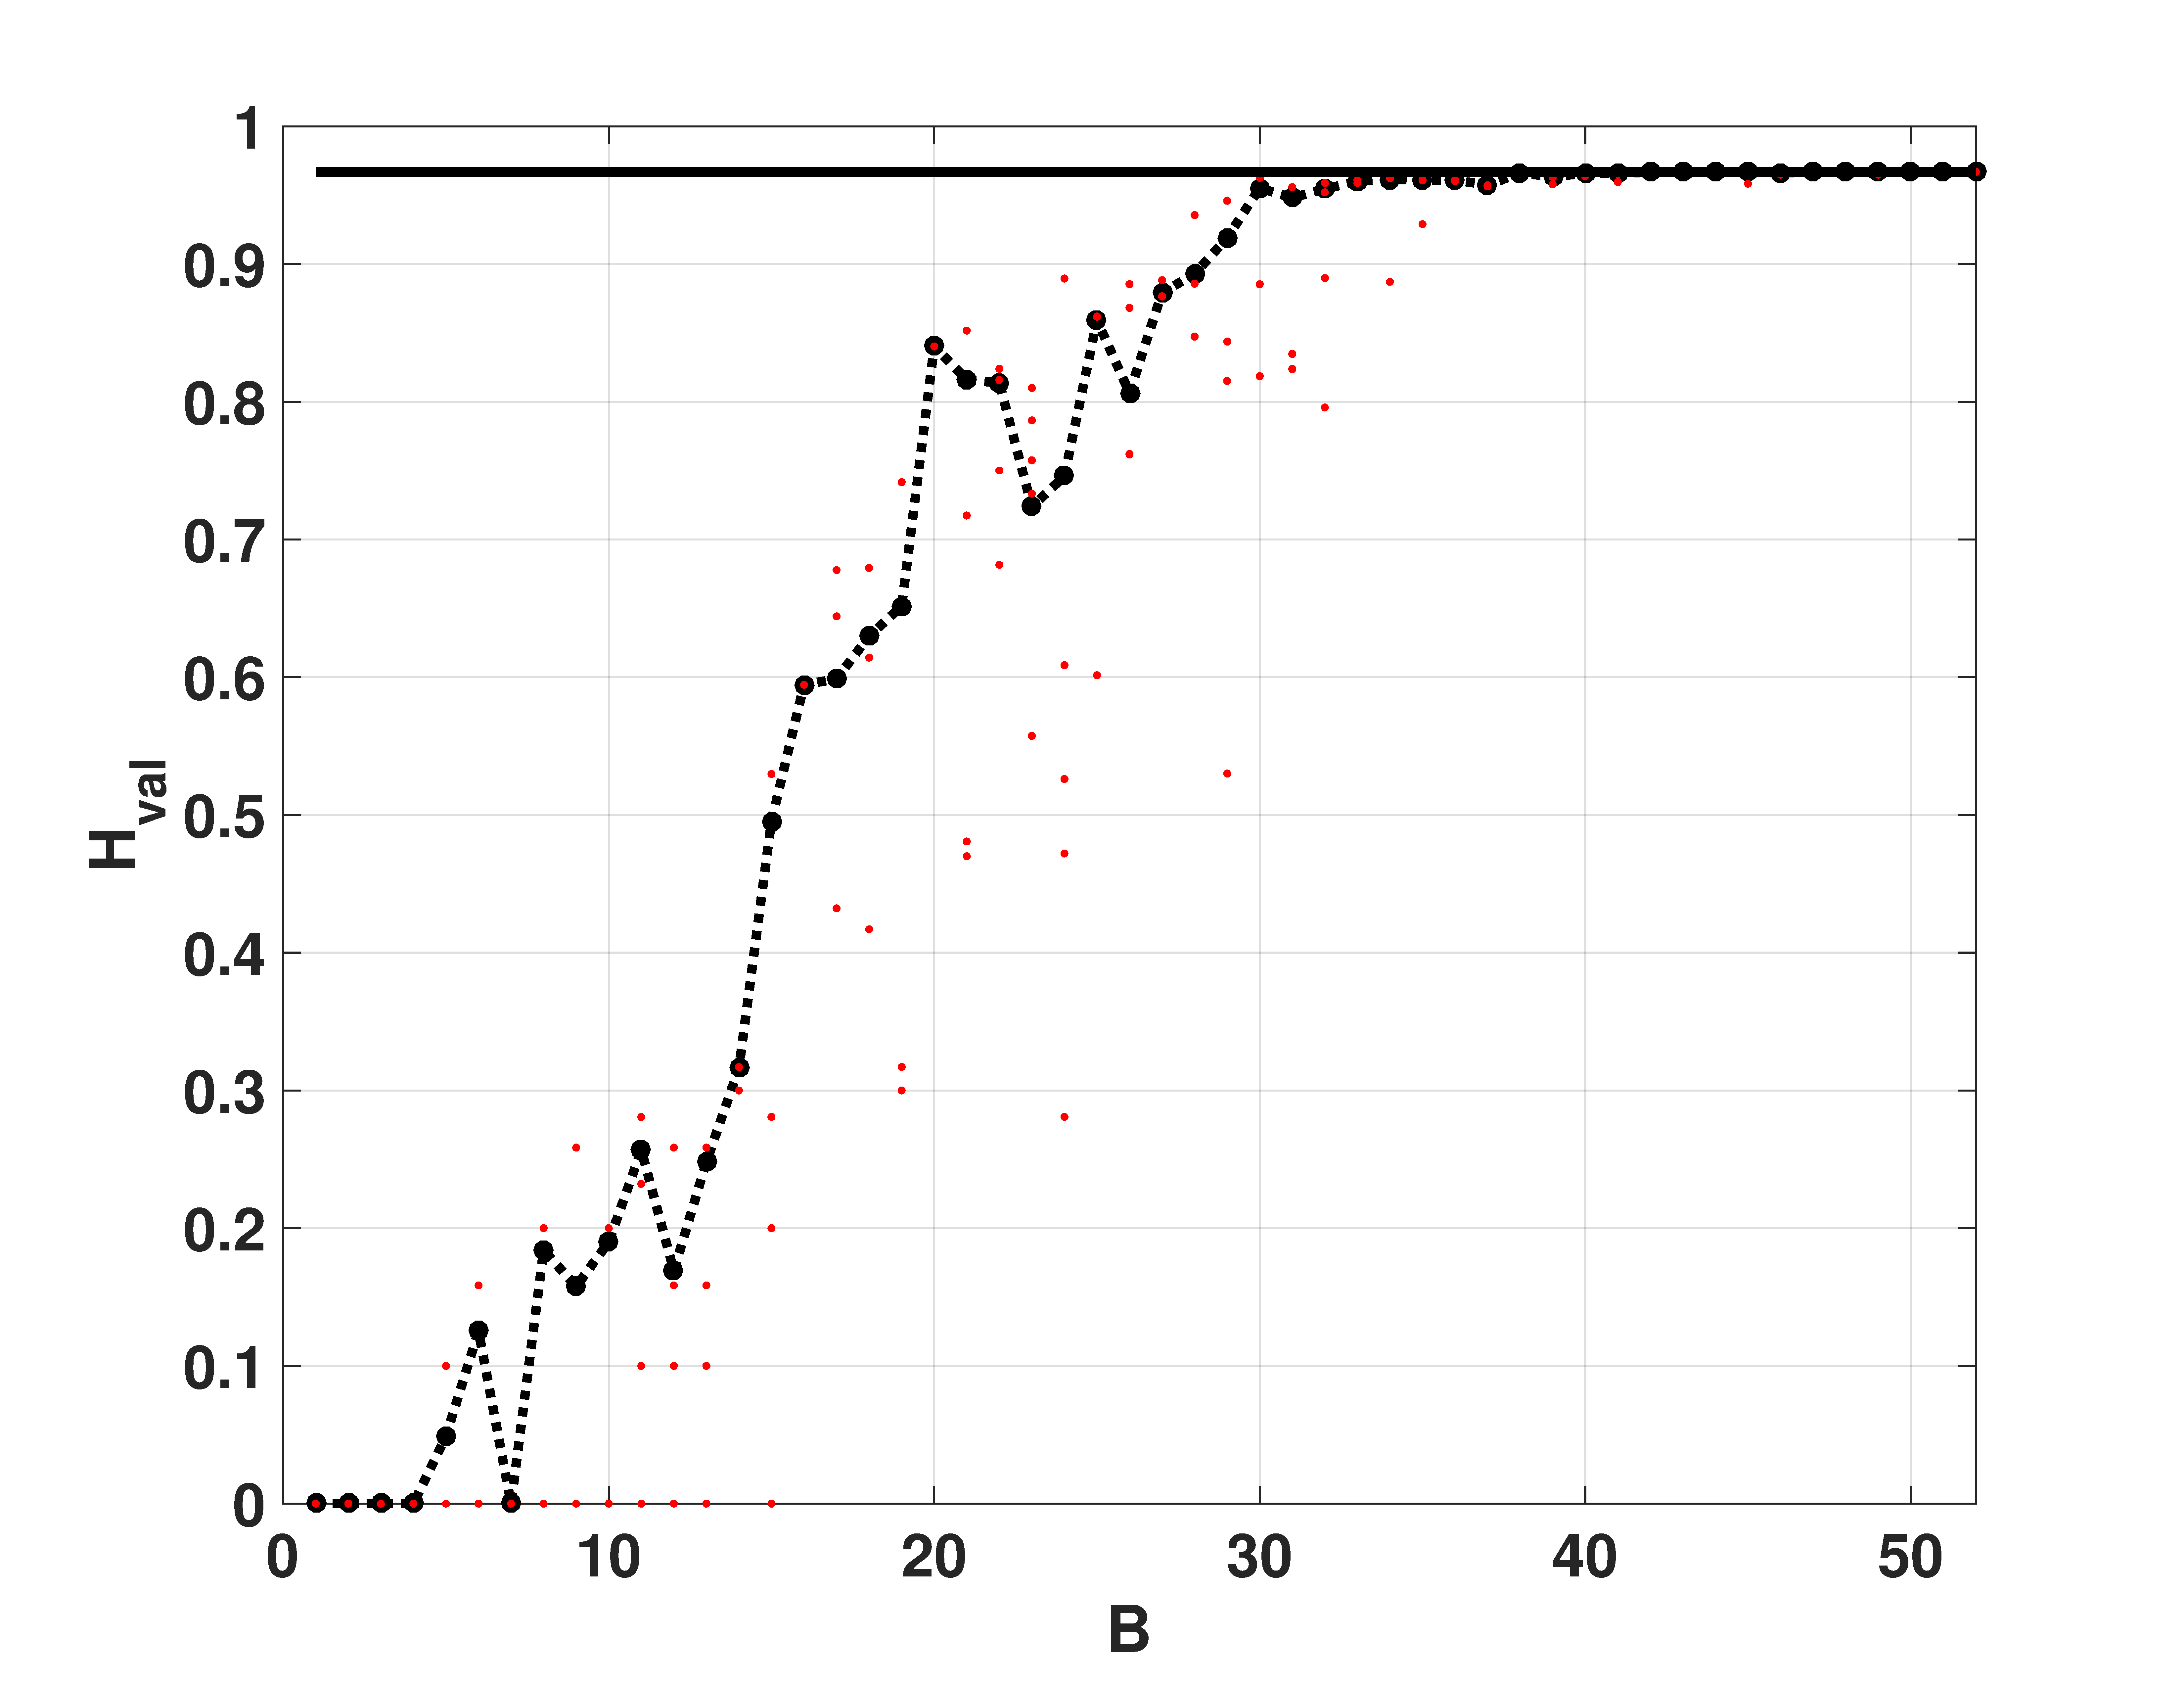
\includegraphics[width=\textwidth]{Hval_Log}
		\caption{$H_{hist}$ vs. $B$}
		\label{fig:Hval_Log}
	\end{subfigure}
	\begin{subfigure}[b]{0.49\textwidth}
		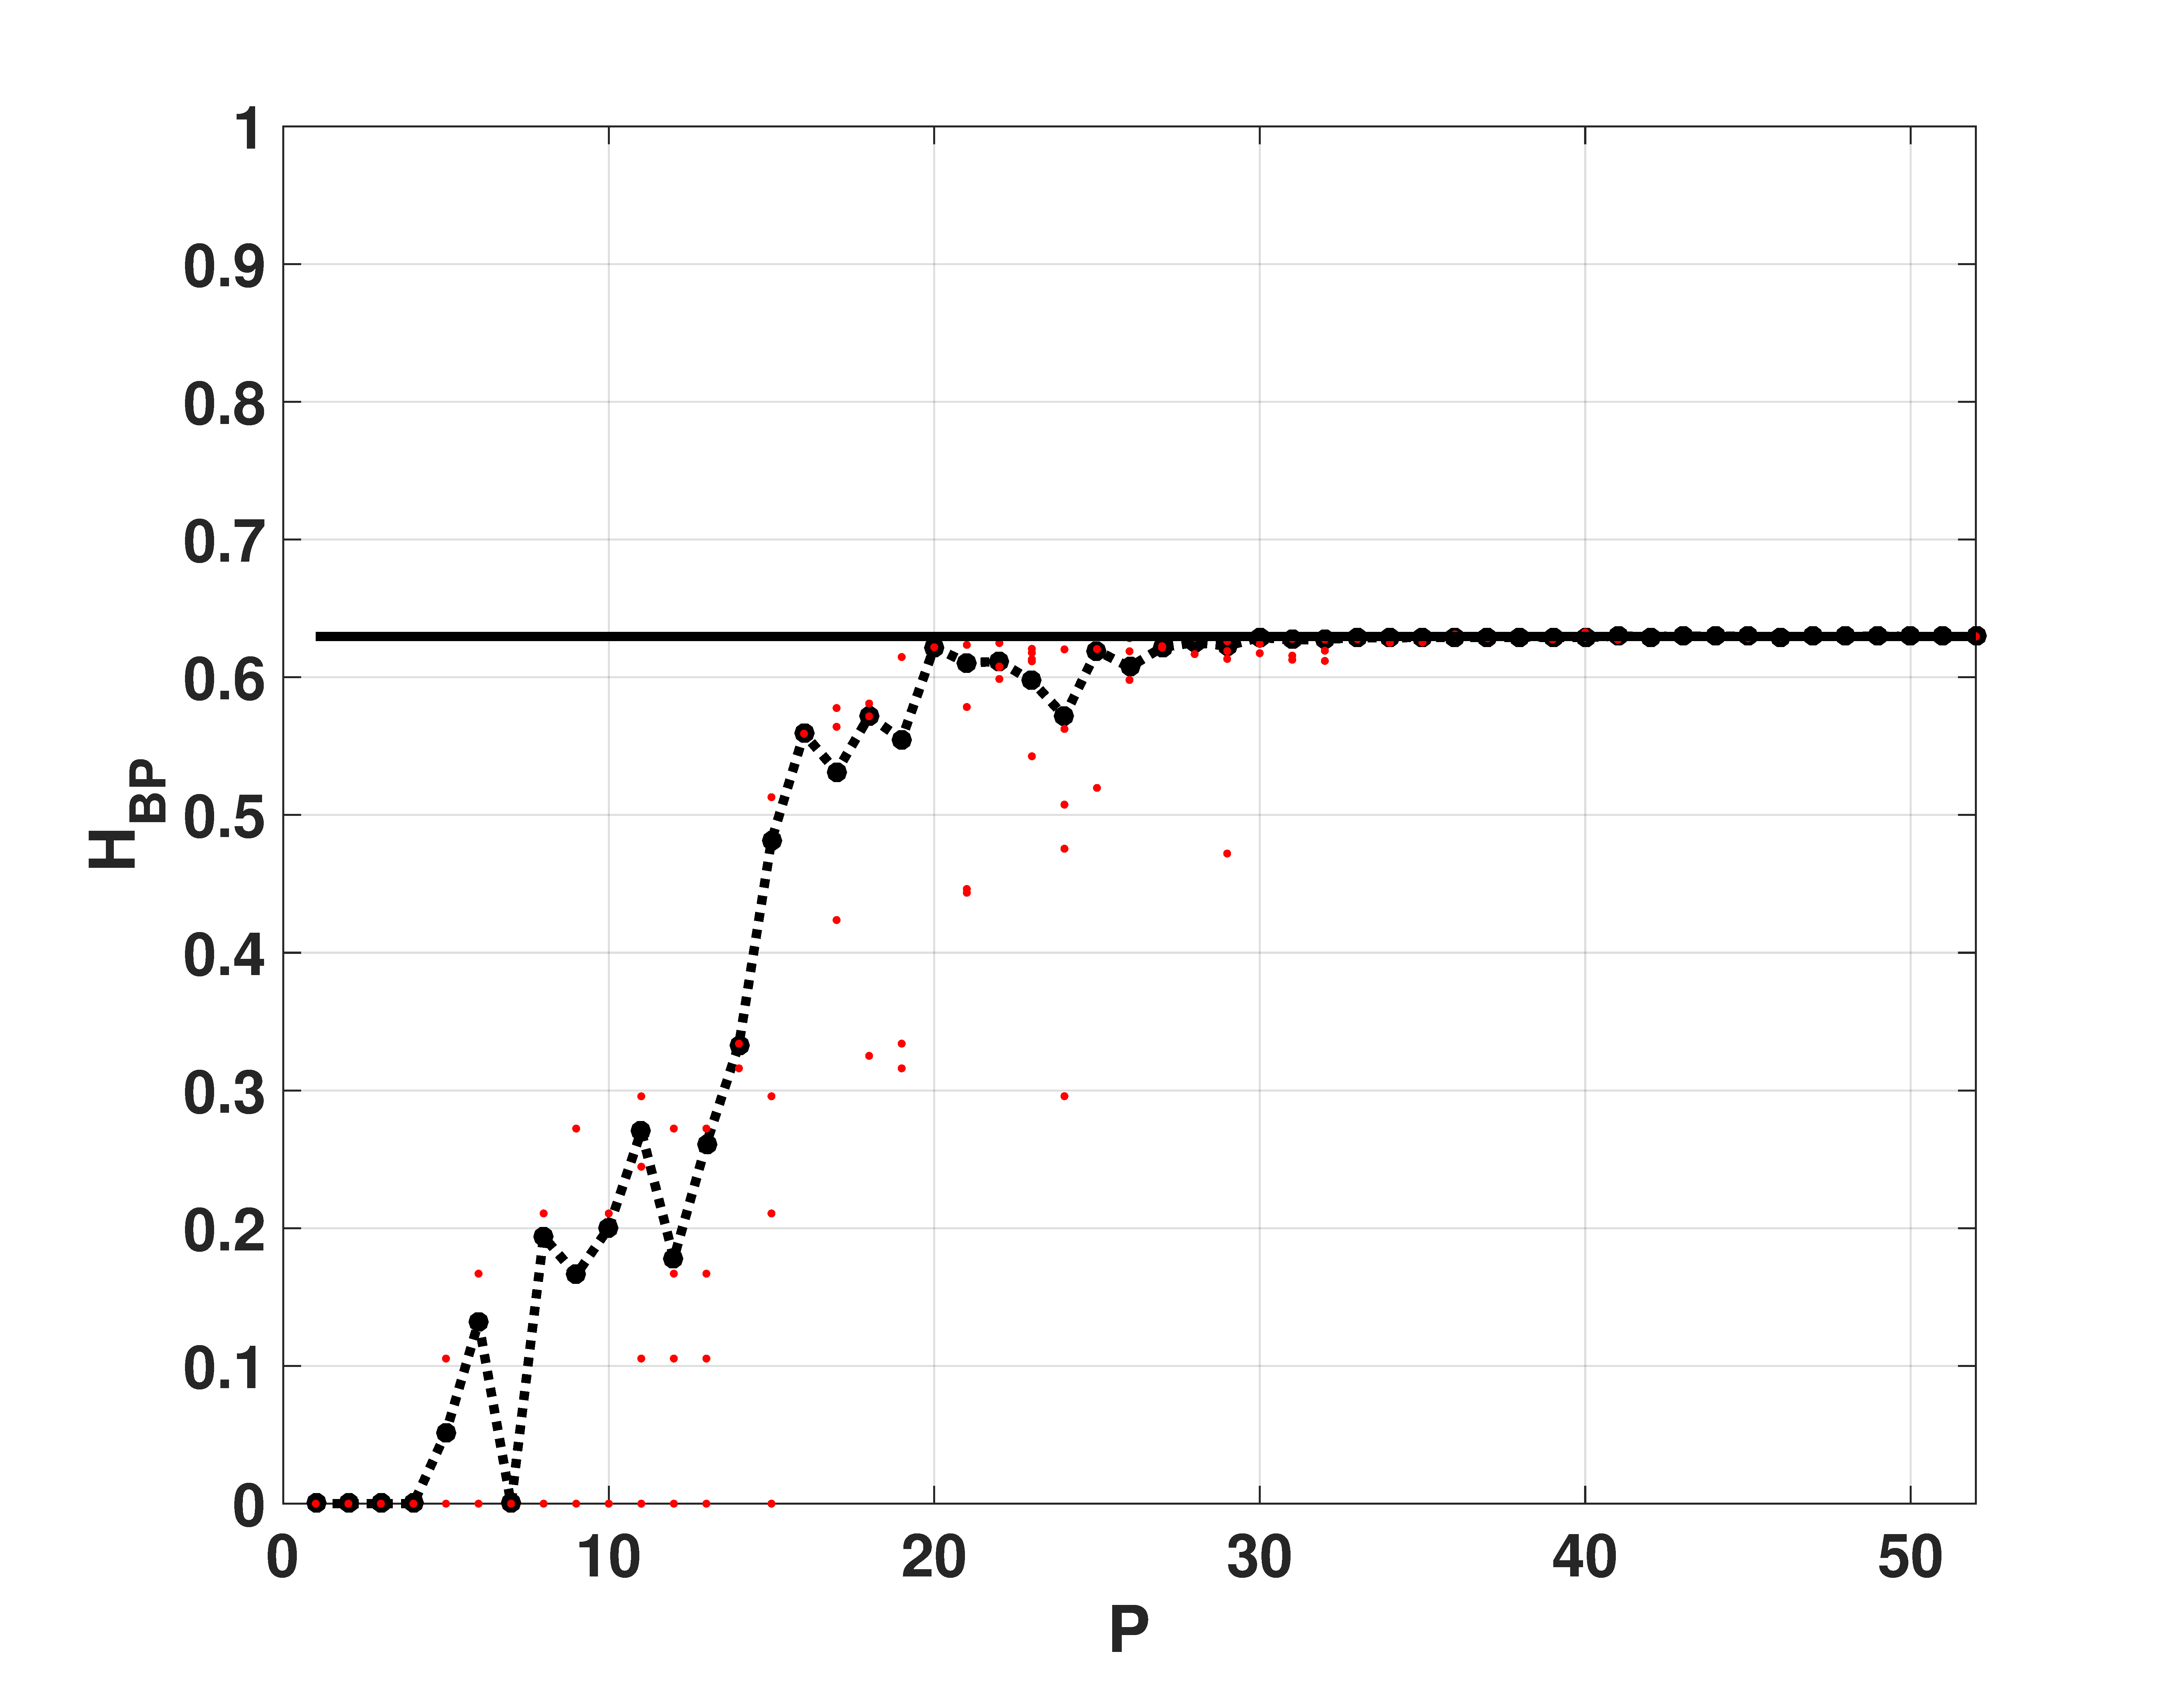
\includegraphics[width=\textwidth]{Hbp_Log}
		\caption{$H_{BP}$ vs. $B$}
		\label{fig:Hbp_Log}
	\end{subfigure}
	\begin{subfigure}[b]{0.49\textwidth}
		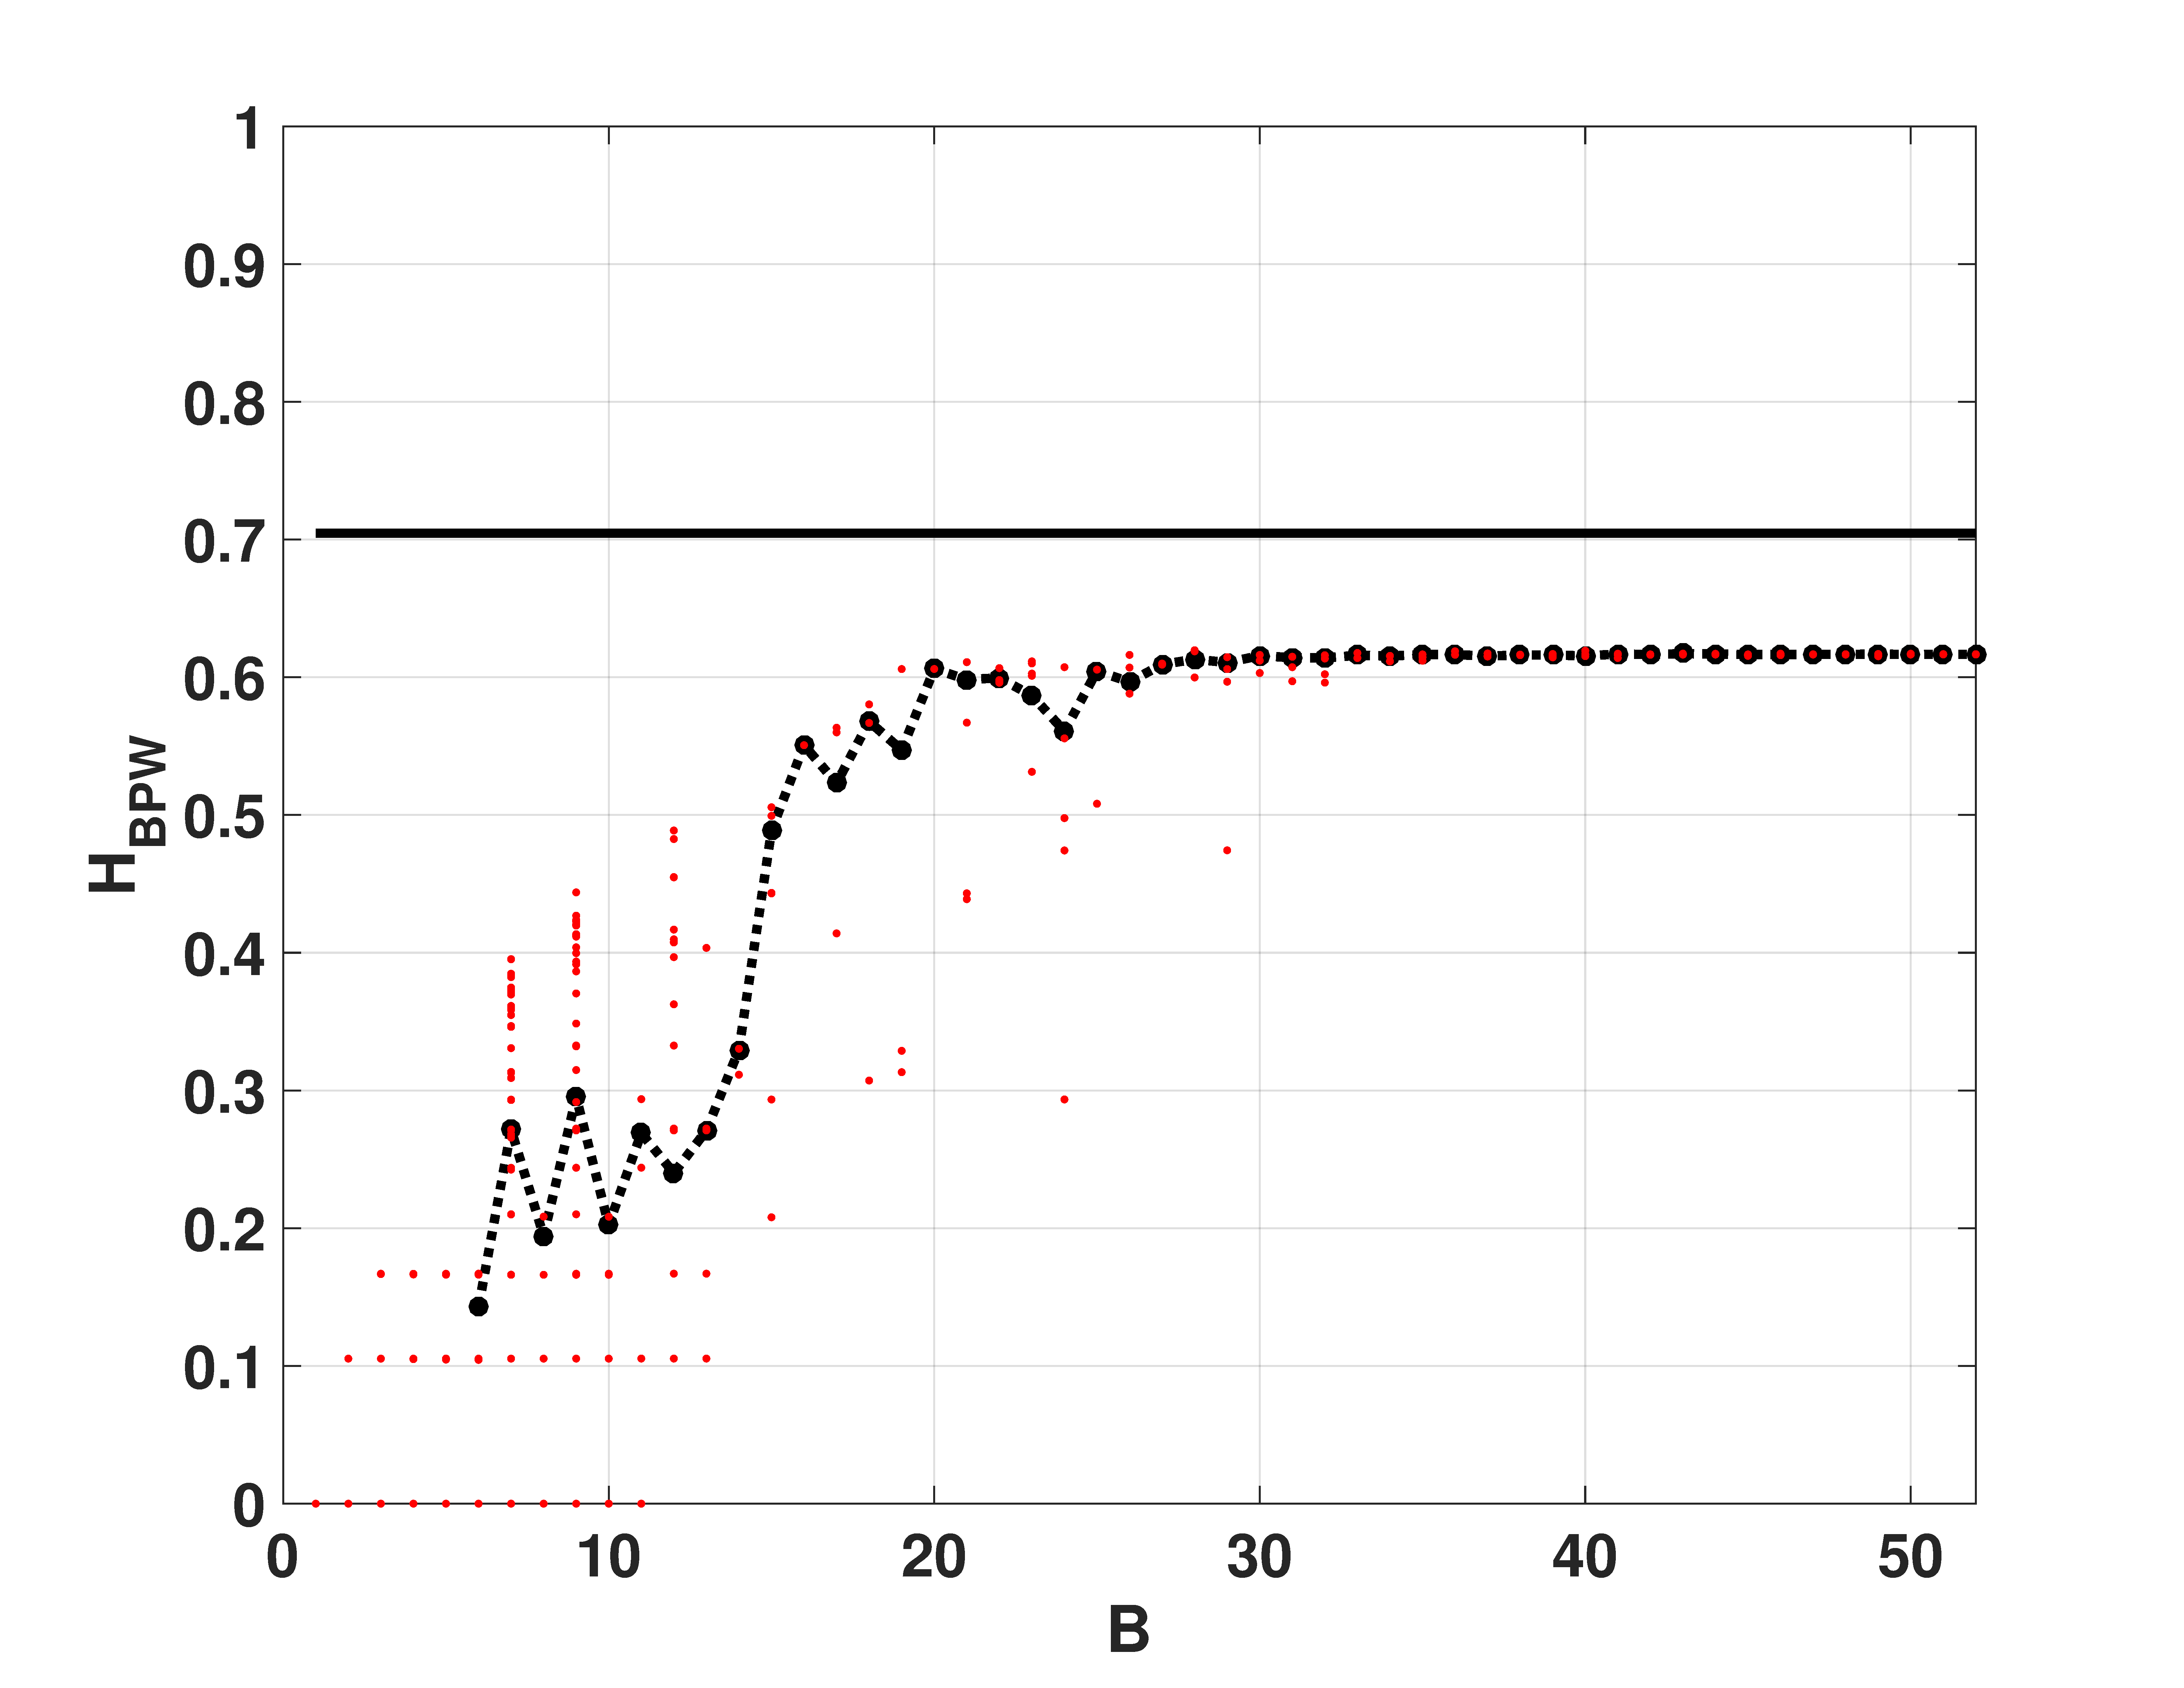
\includegraphics[width=\textwidth]{Hbpw_Log}
		\caption{$H_{BPW}$ vs. $B$}
		\label{fig:Hbpw_Log}
	\end{subfigure}
	\begin{subfigure}[b]{0.49\textwidth}
		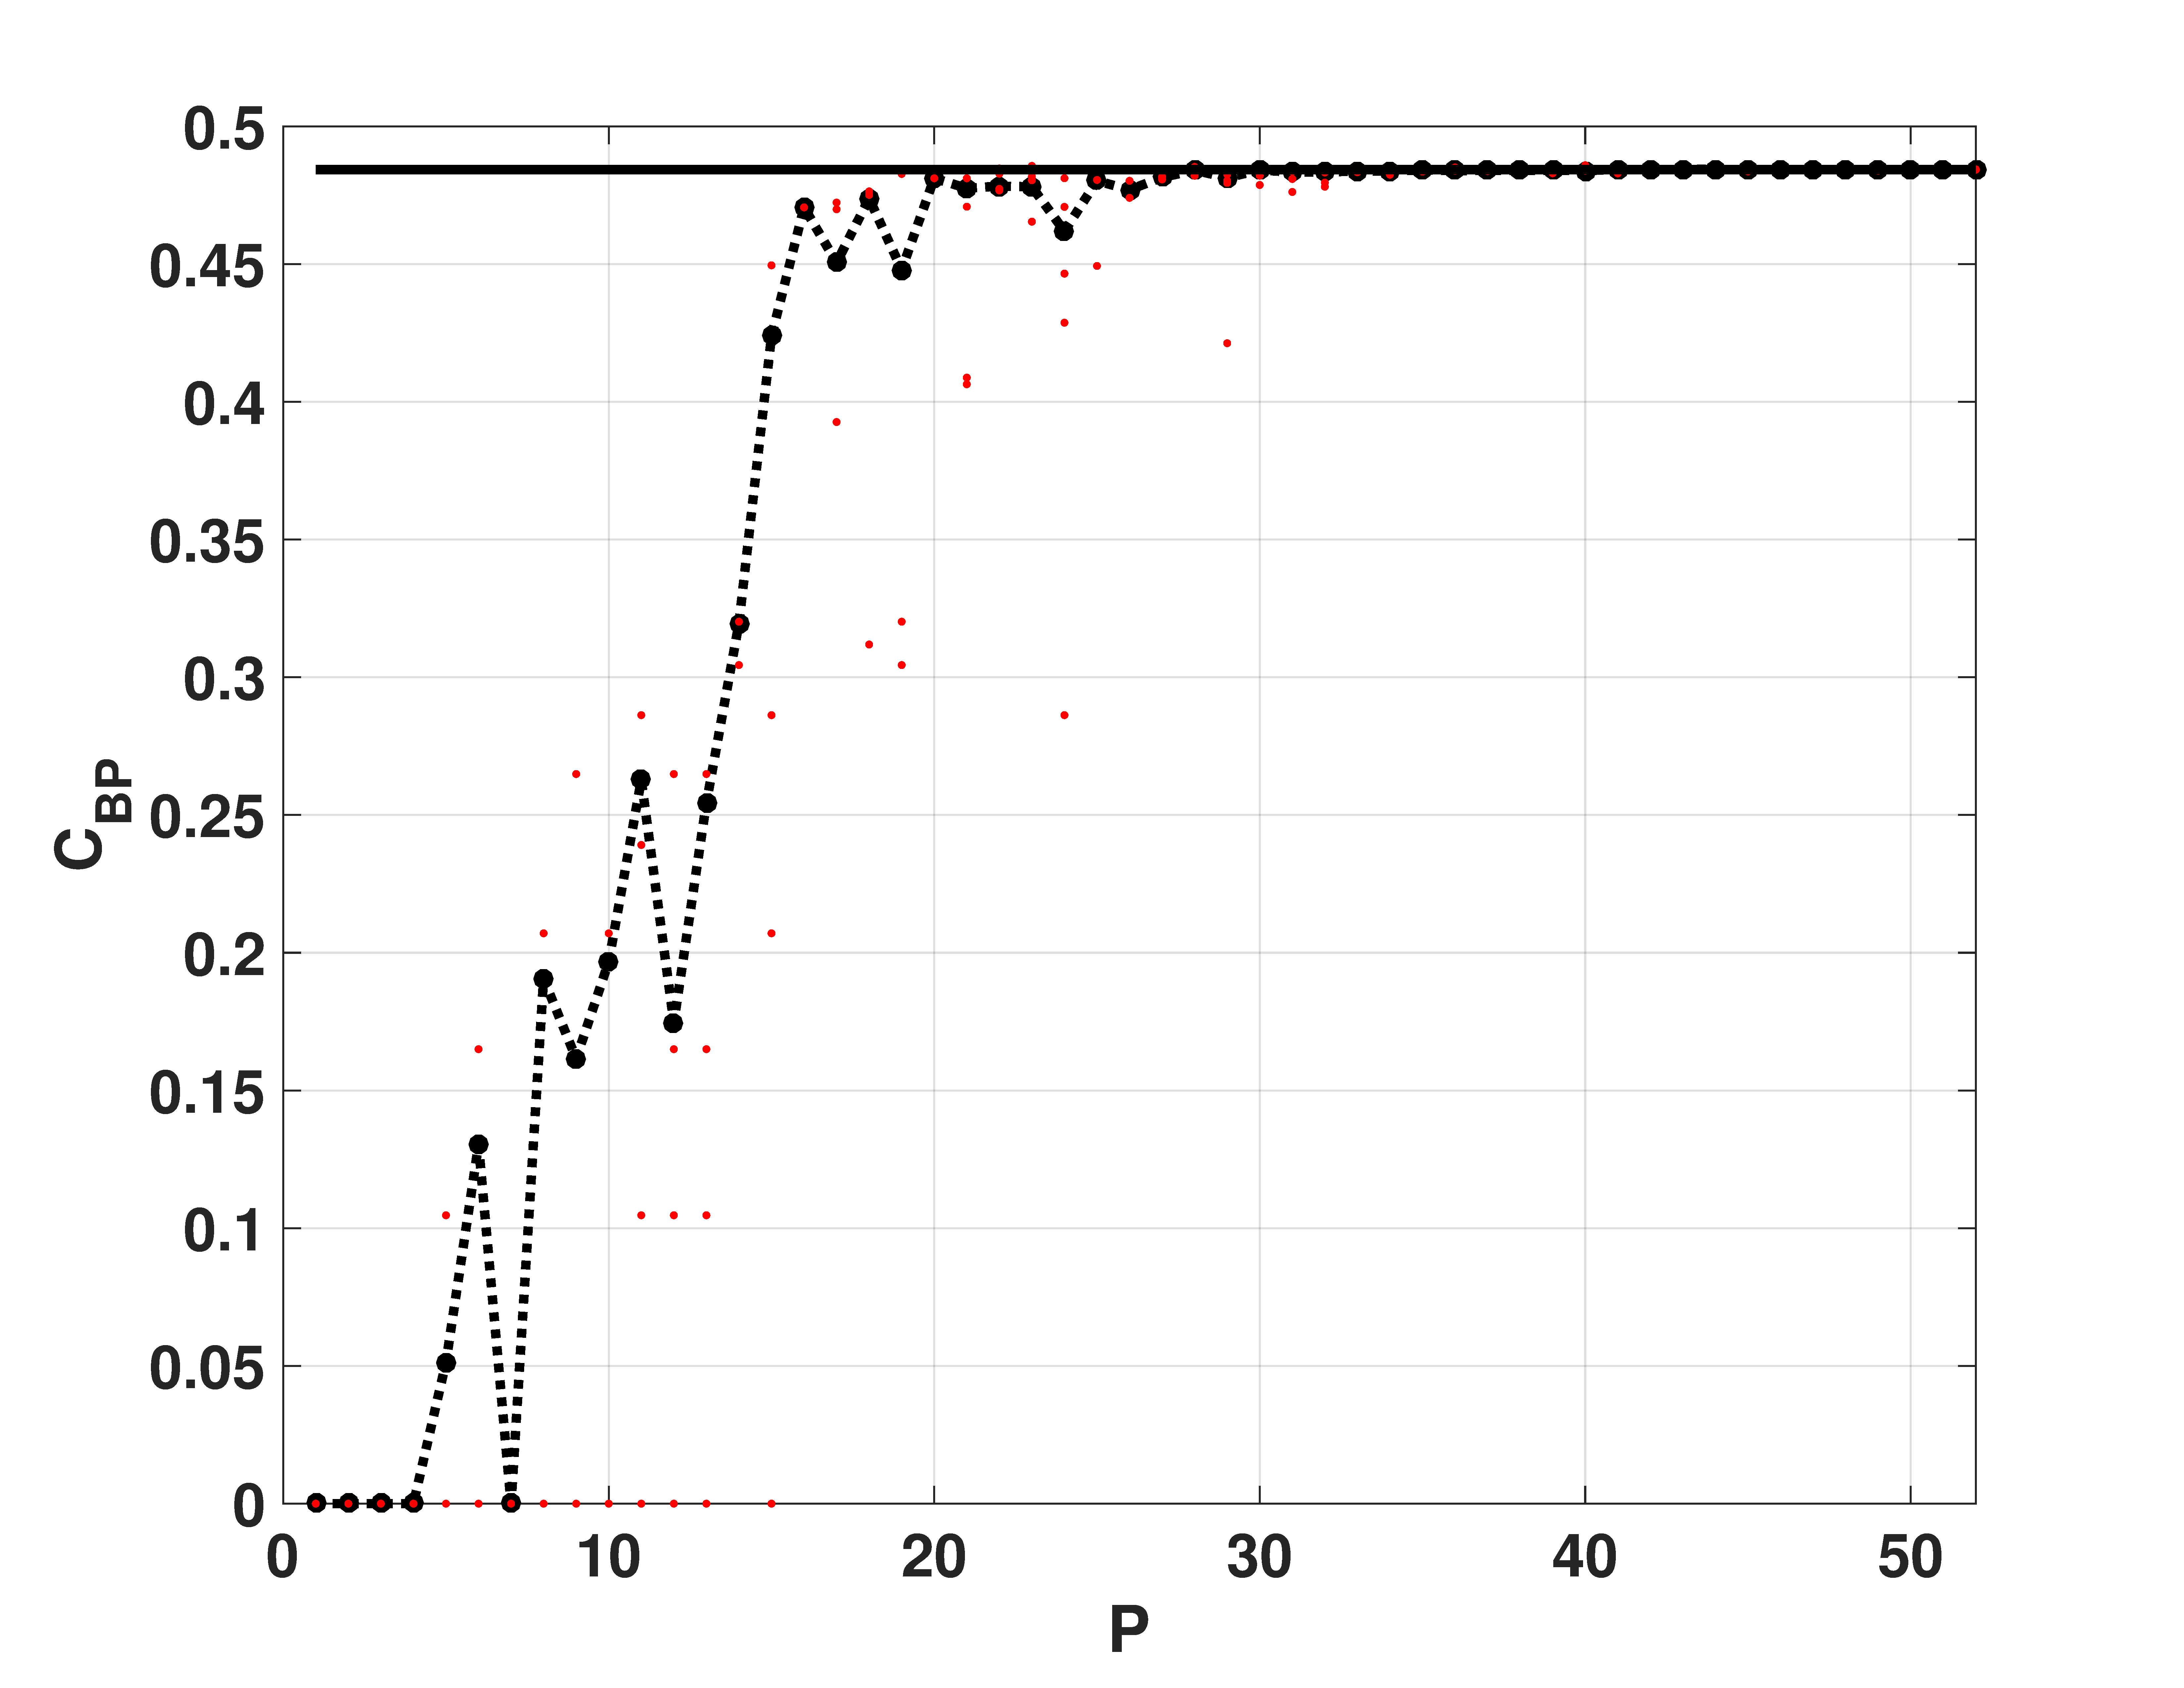
\includegraphics[width=\textwidth]{Cbp_Log}
		\caption{$C_{BP}$ vs. $B$}
		\label{fig:Cbp_Log}
	\end{subfigure}
	\begin{subfigure}[b]{0.49\textwidth}
		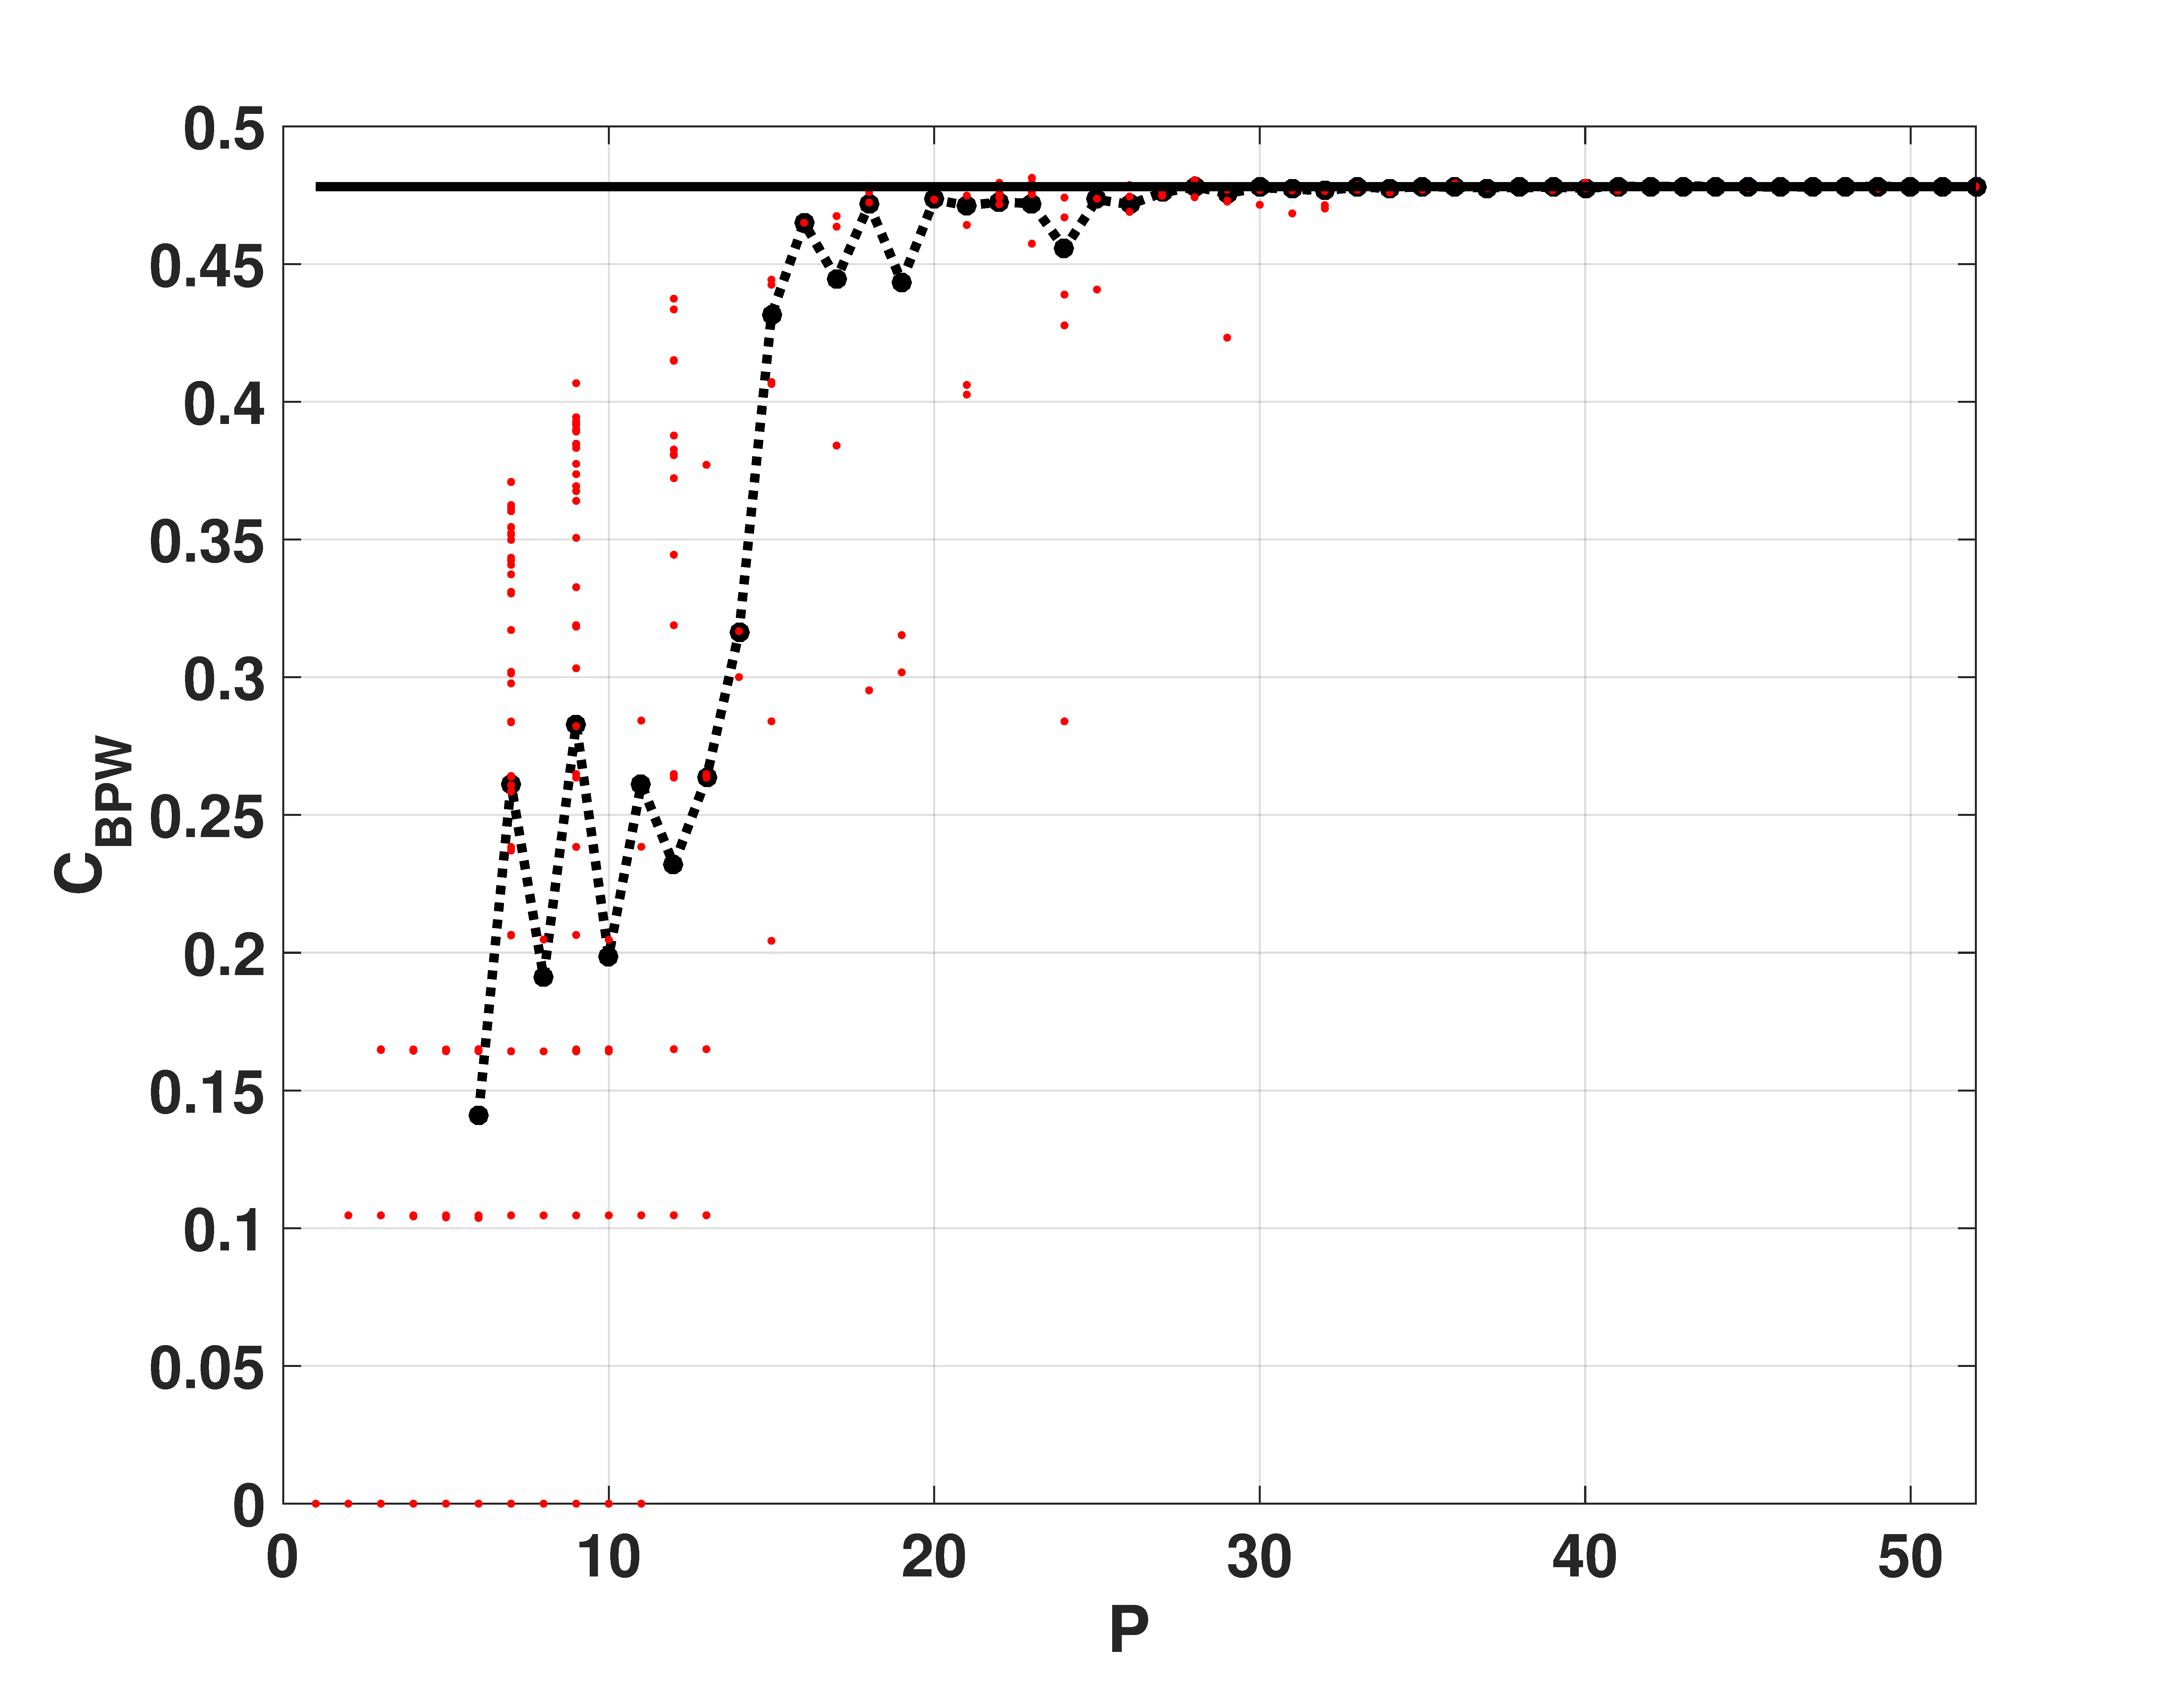
\includegraphics[width=\textwidth]{Cbpw_Log}
		\caption{$C_{BPW}$ vs. $B$}
		\label{fig:Cbpw_Log}
	\end{subfigure}
	\begin{subfigure}[b]{0.49\textwidth}
		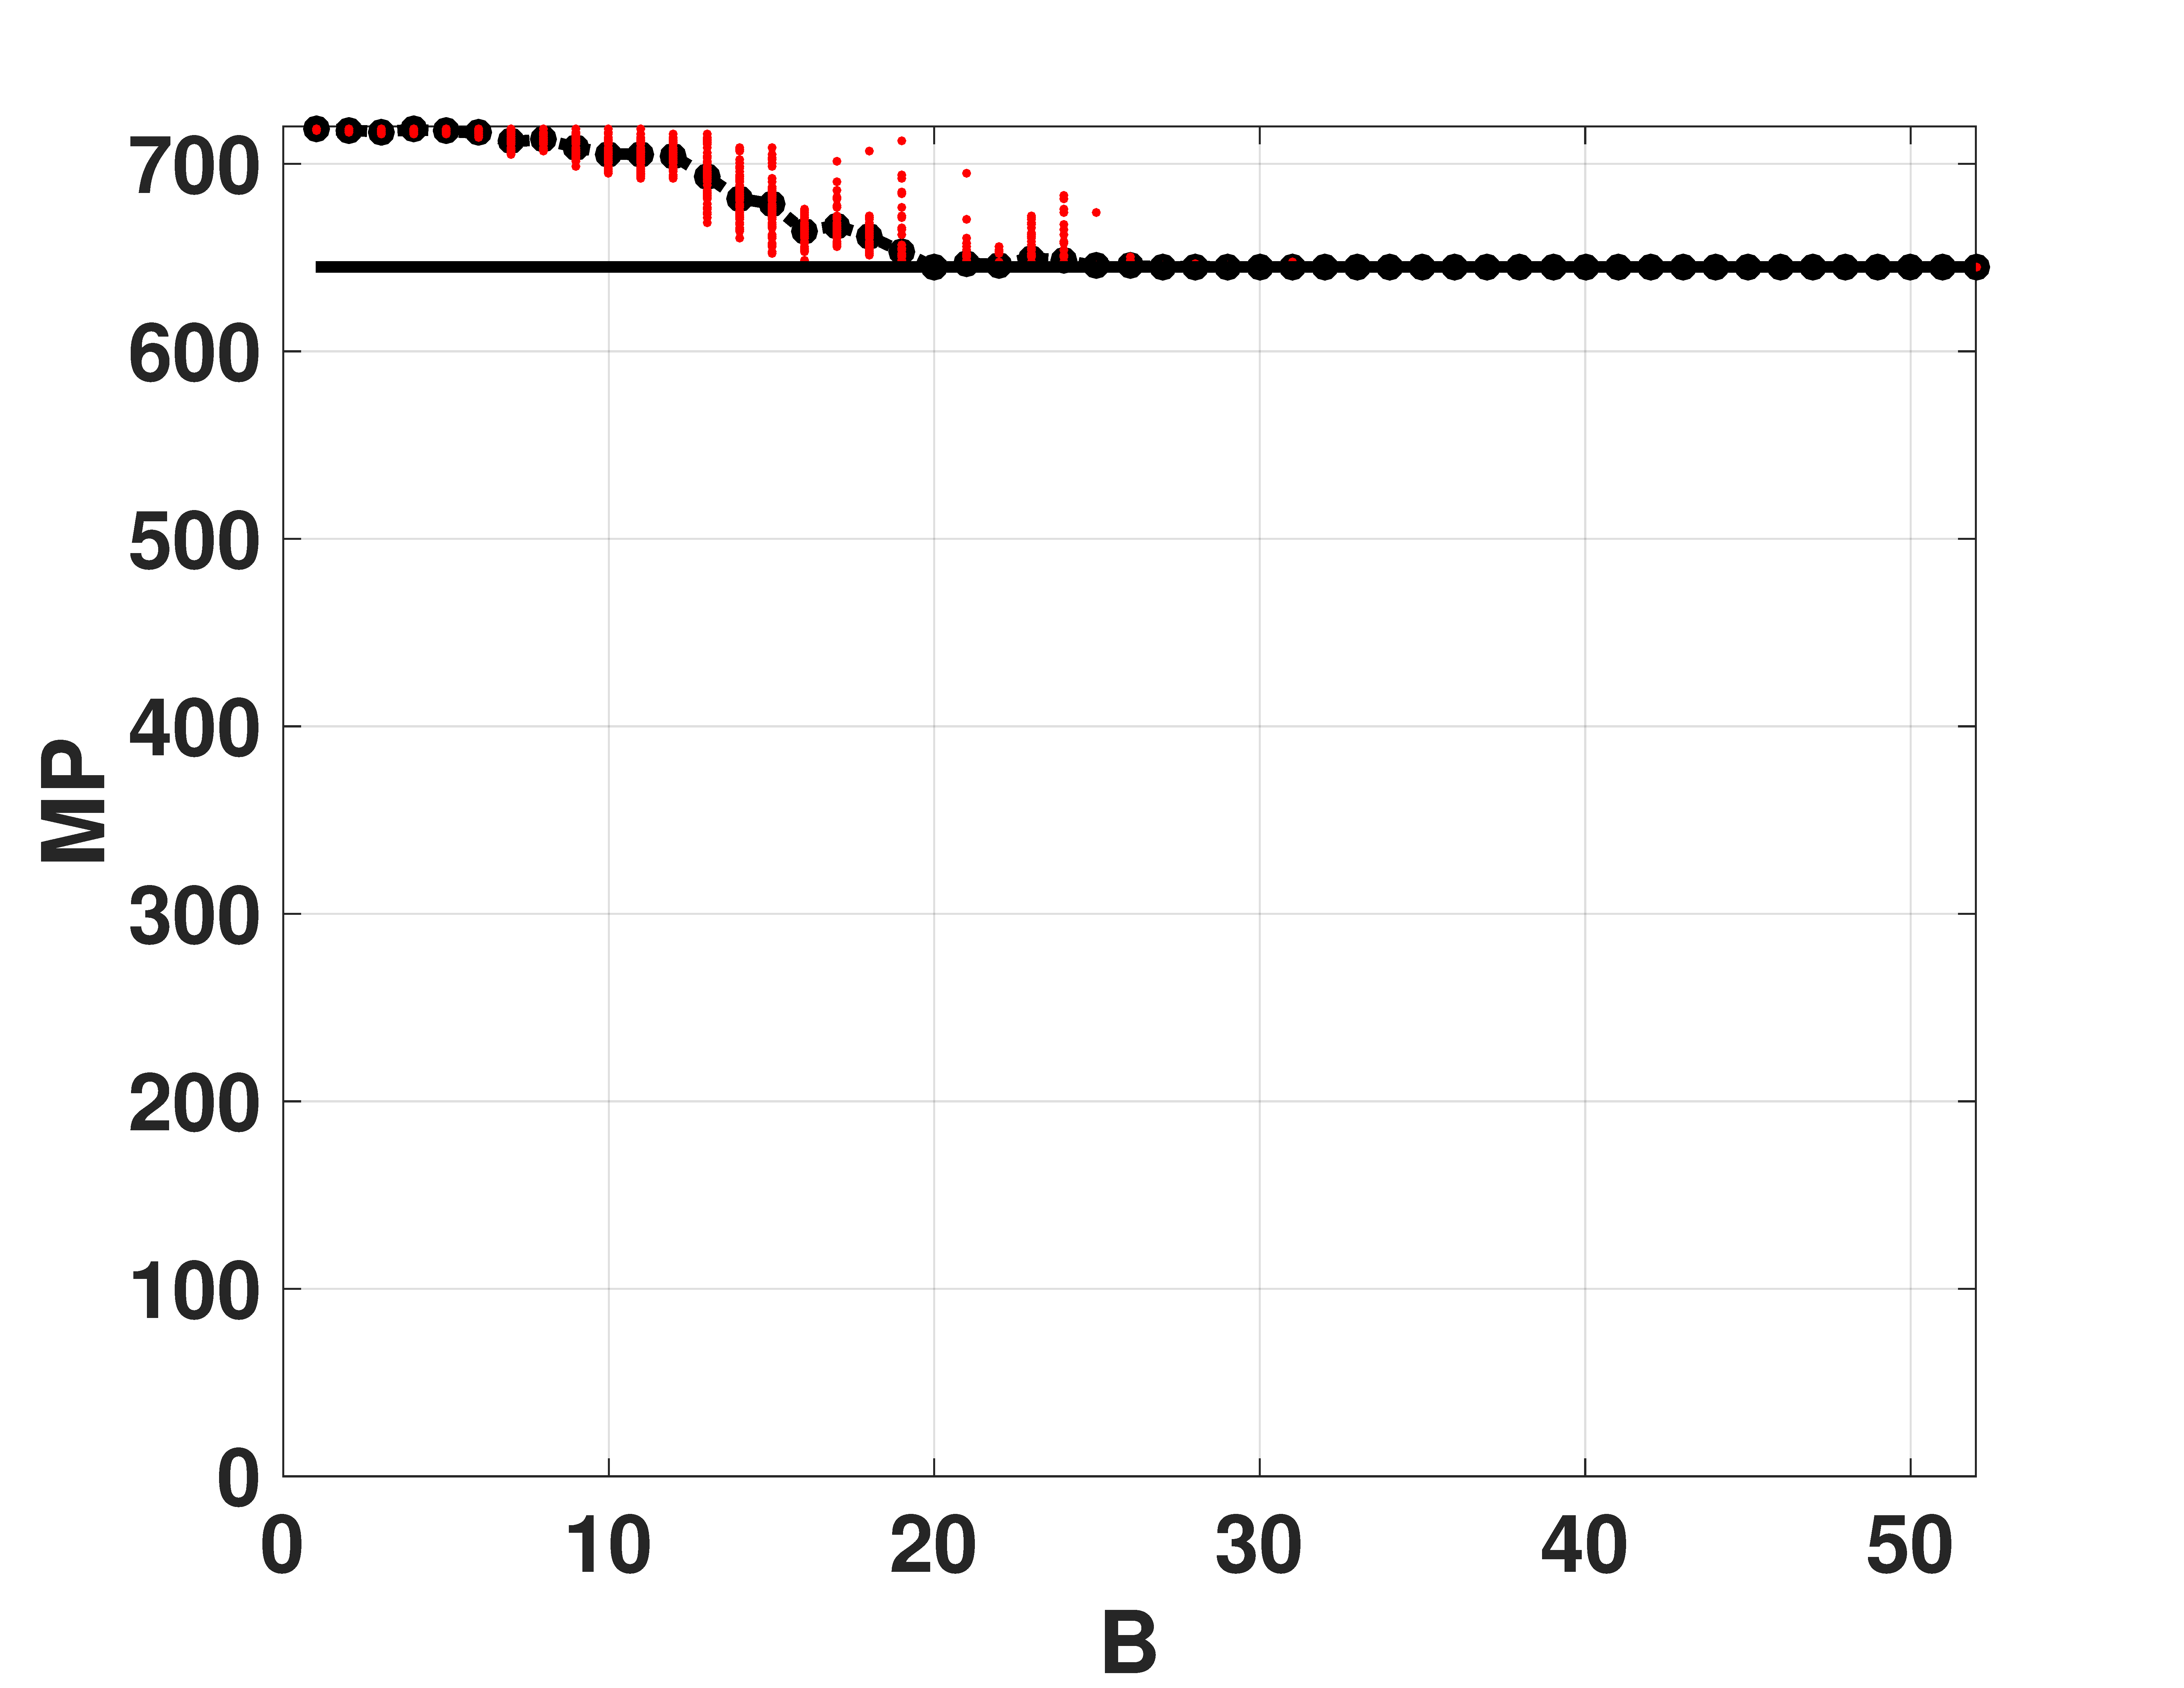
\includegraphics[width=\textwidth]{MP_Log}
		\caption{MP vs. $B$}
		\label{fig:MP_Log}
	\end{subfigure}
	\caption{Statistical properties for LOG map as function of $B$}
	\label{fig:LOG_QuantiB}
\end{figure}

The same results are shown in double entropy planes with the precision as parameter (Fig. \ref{fig:LOG_HH} (a) without amplitude contributions and \ref{fig:LOG_HH} (b) with amplitude contributions).
These figures show: $100$ red points for each fixed-point precision ($B$) and in black their average (dashed black line connecting black dots), $100$ blue dots that are the results of each run in floating-point and the black star is their average.
Here, the $100$ blue points and their average are overlapped.

As expected, the fixed-point architecture implementation converges to the floating-point value as $B$ increases.
For both, $H_{hist} \times H_{BP}$ and $H_{hist} \times H_{BPW}$, from $B=20$, $H_{hist}$ improves but $H_{BP}$ and $H_{BPW}$ remains constant.
It can be seen that the distribution of values reaches high values ($\left\langle H_{hist}\right\rangle =0.9669$) but their mixing is poor ($\left\langle H_{BP}\right\rangle =0.6269$).

\begin{figure}[htpb]
	\centering
	\begin{subfigure}[b]{0.49\textwidth}
		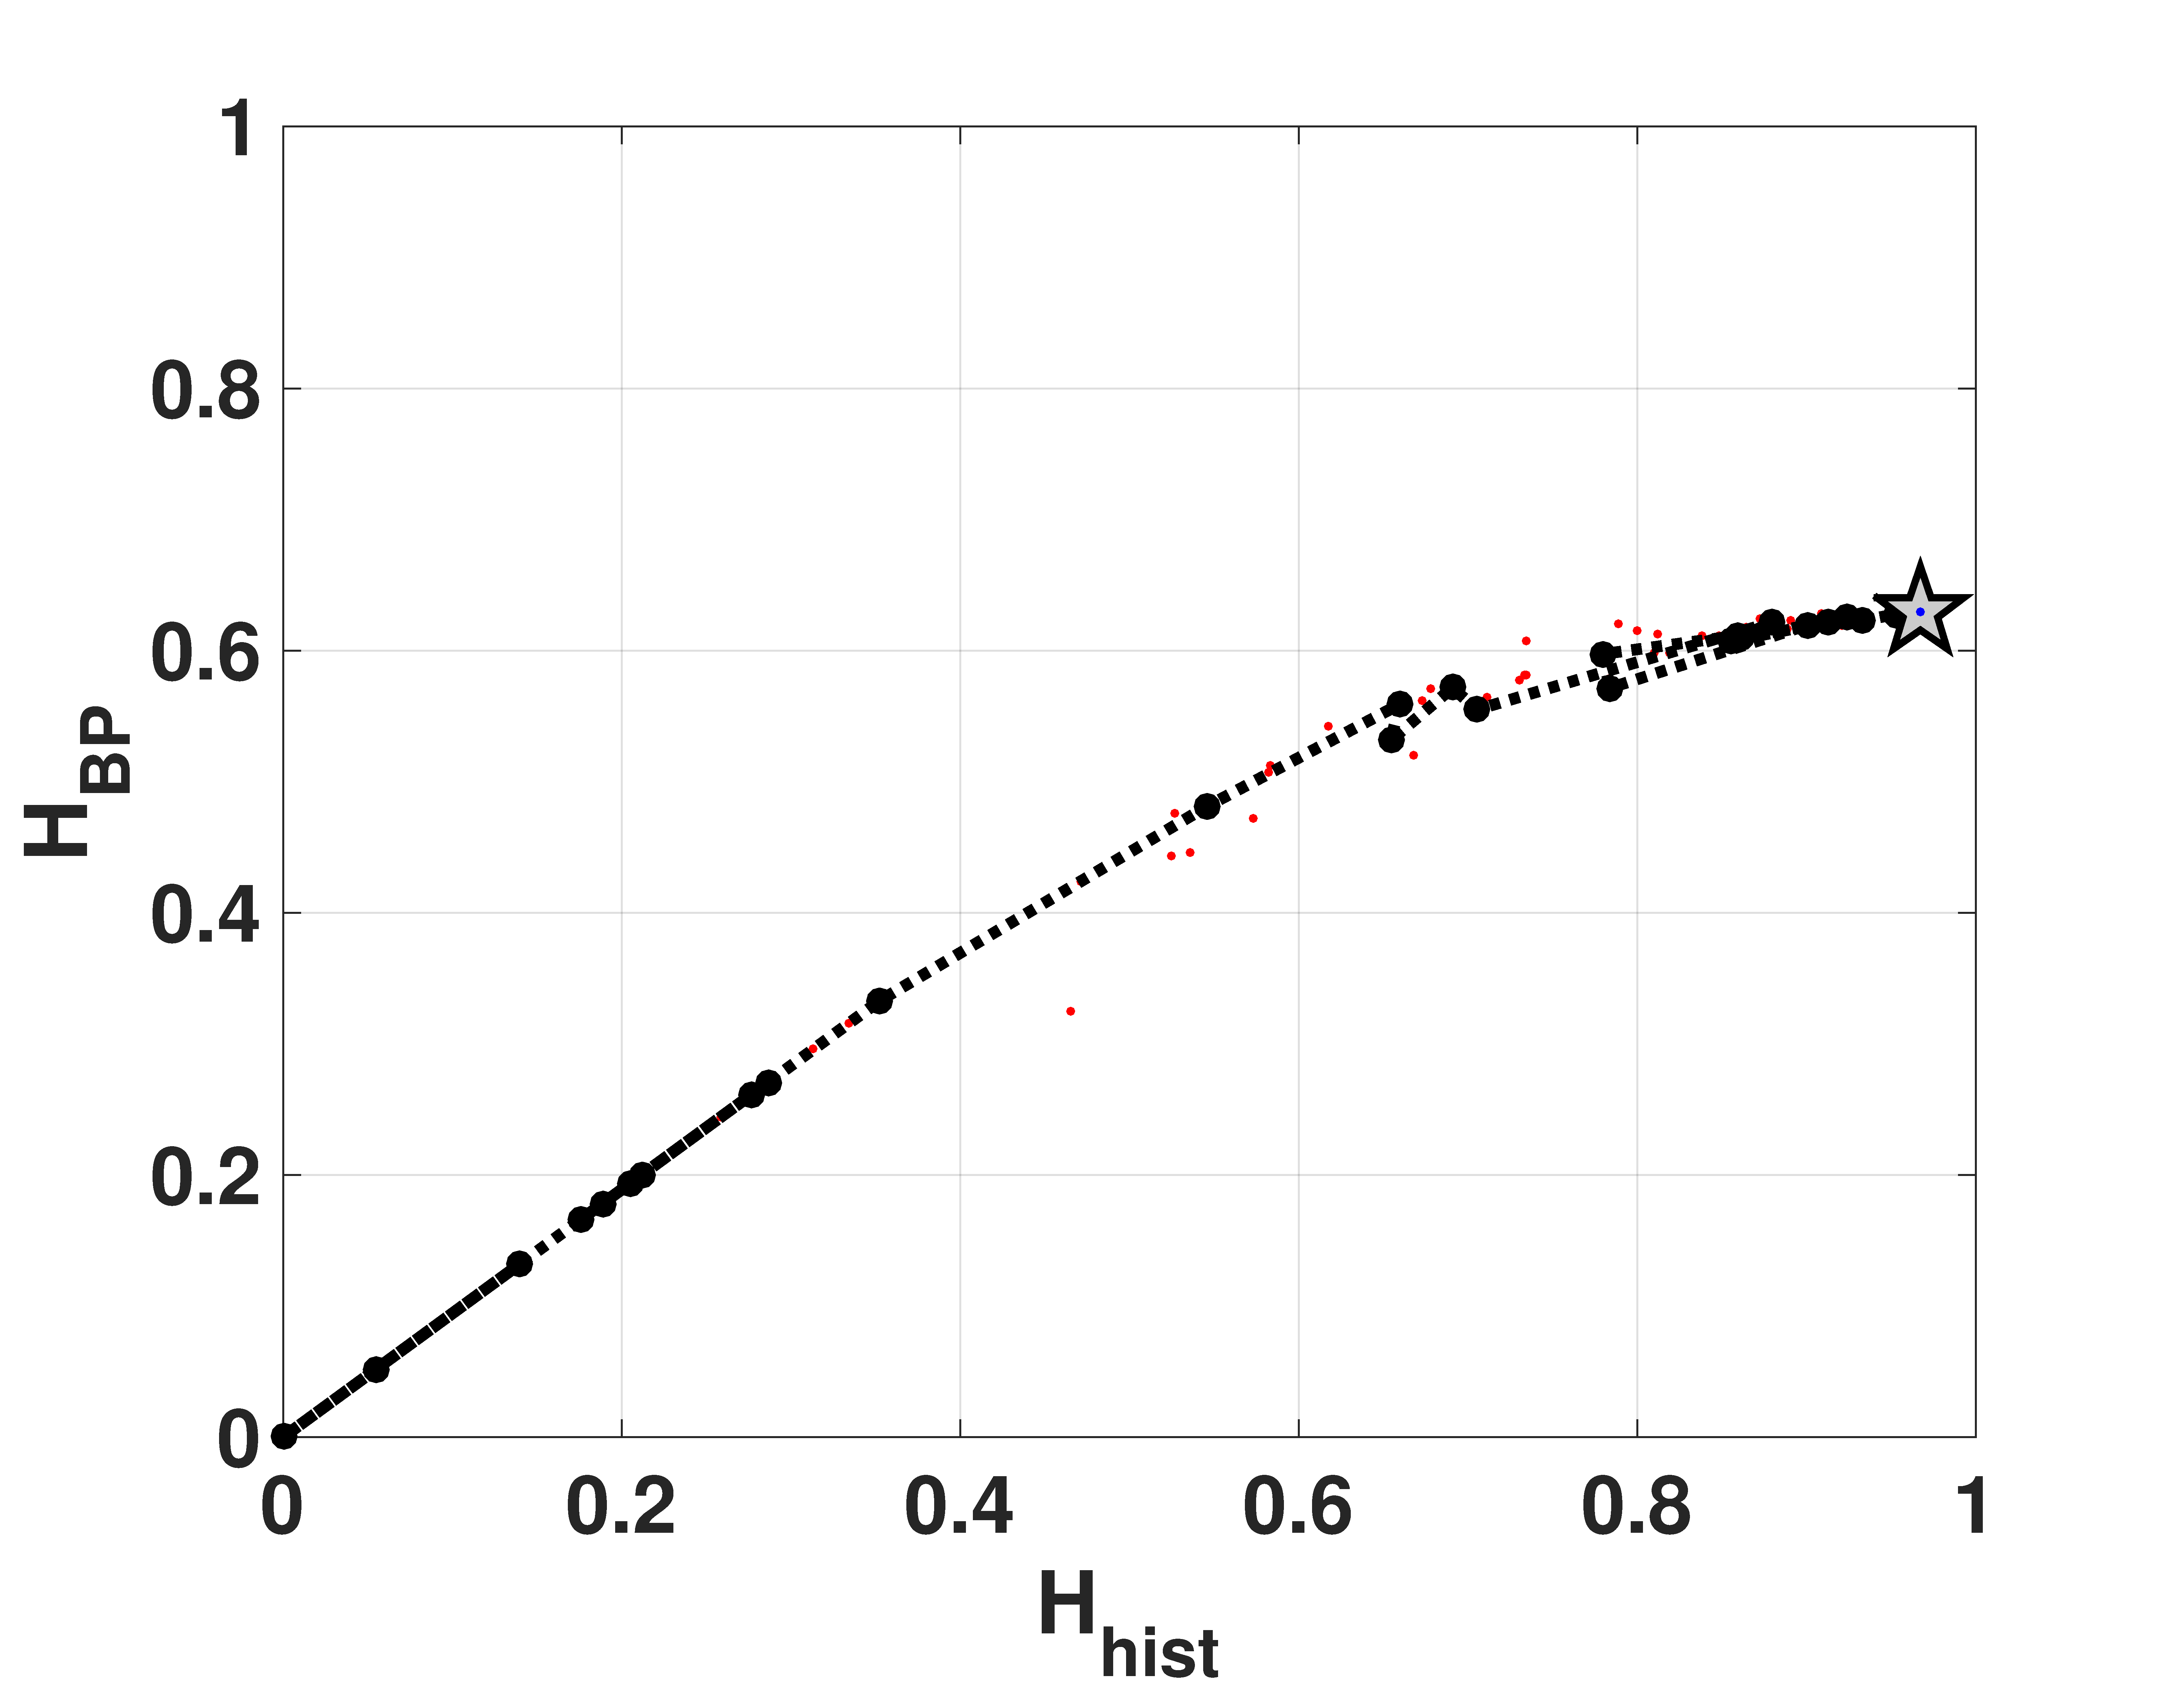
\includegraphics[width=\textwidth]{HbpHval_Log}
		\caption{$H_{hist} \times H_{BP}$}
		\label{fig:HbpHval_Log}
	\end{subfigure}
	\begin{subfigure}[b]{0.49\textwidth}
		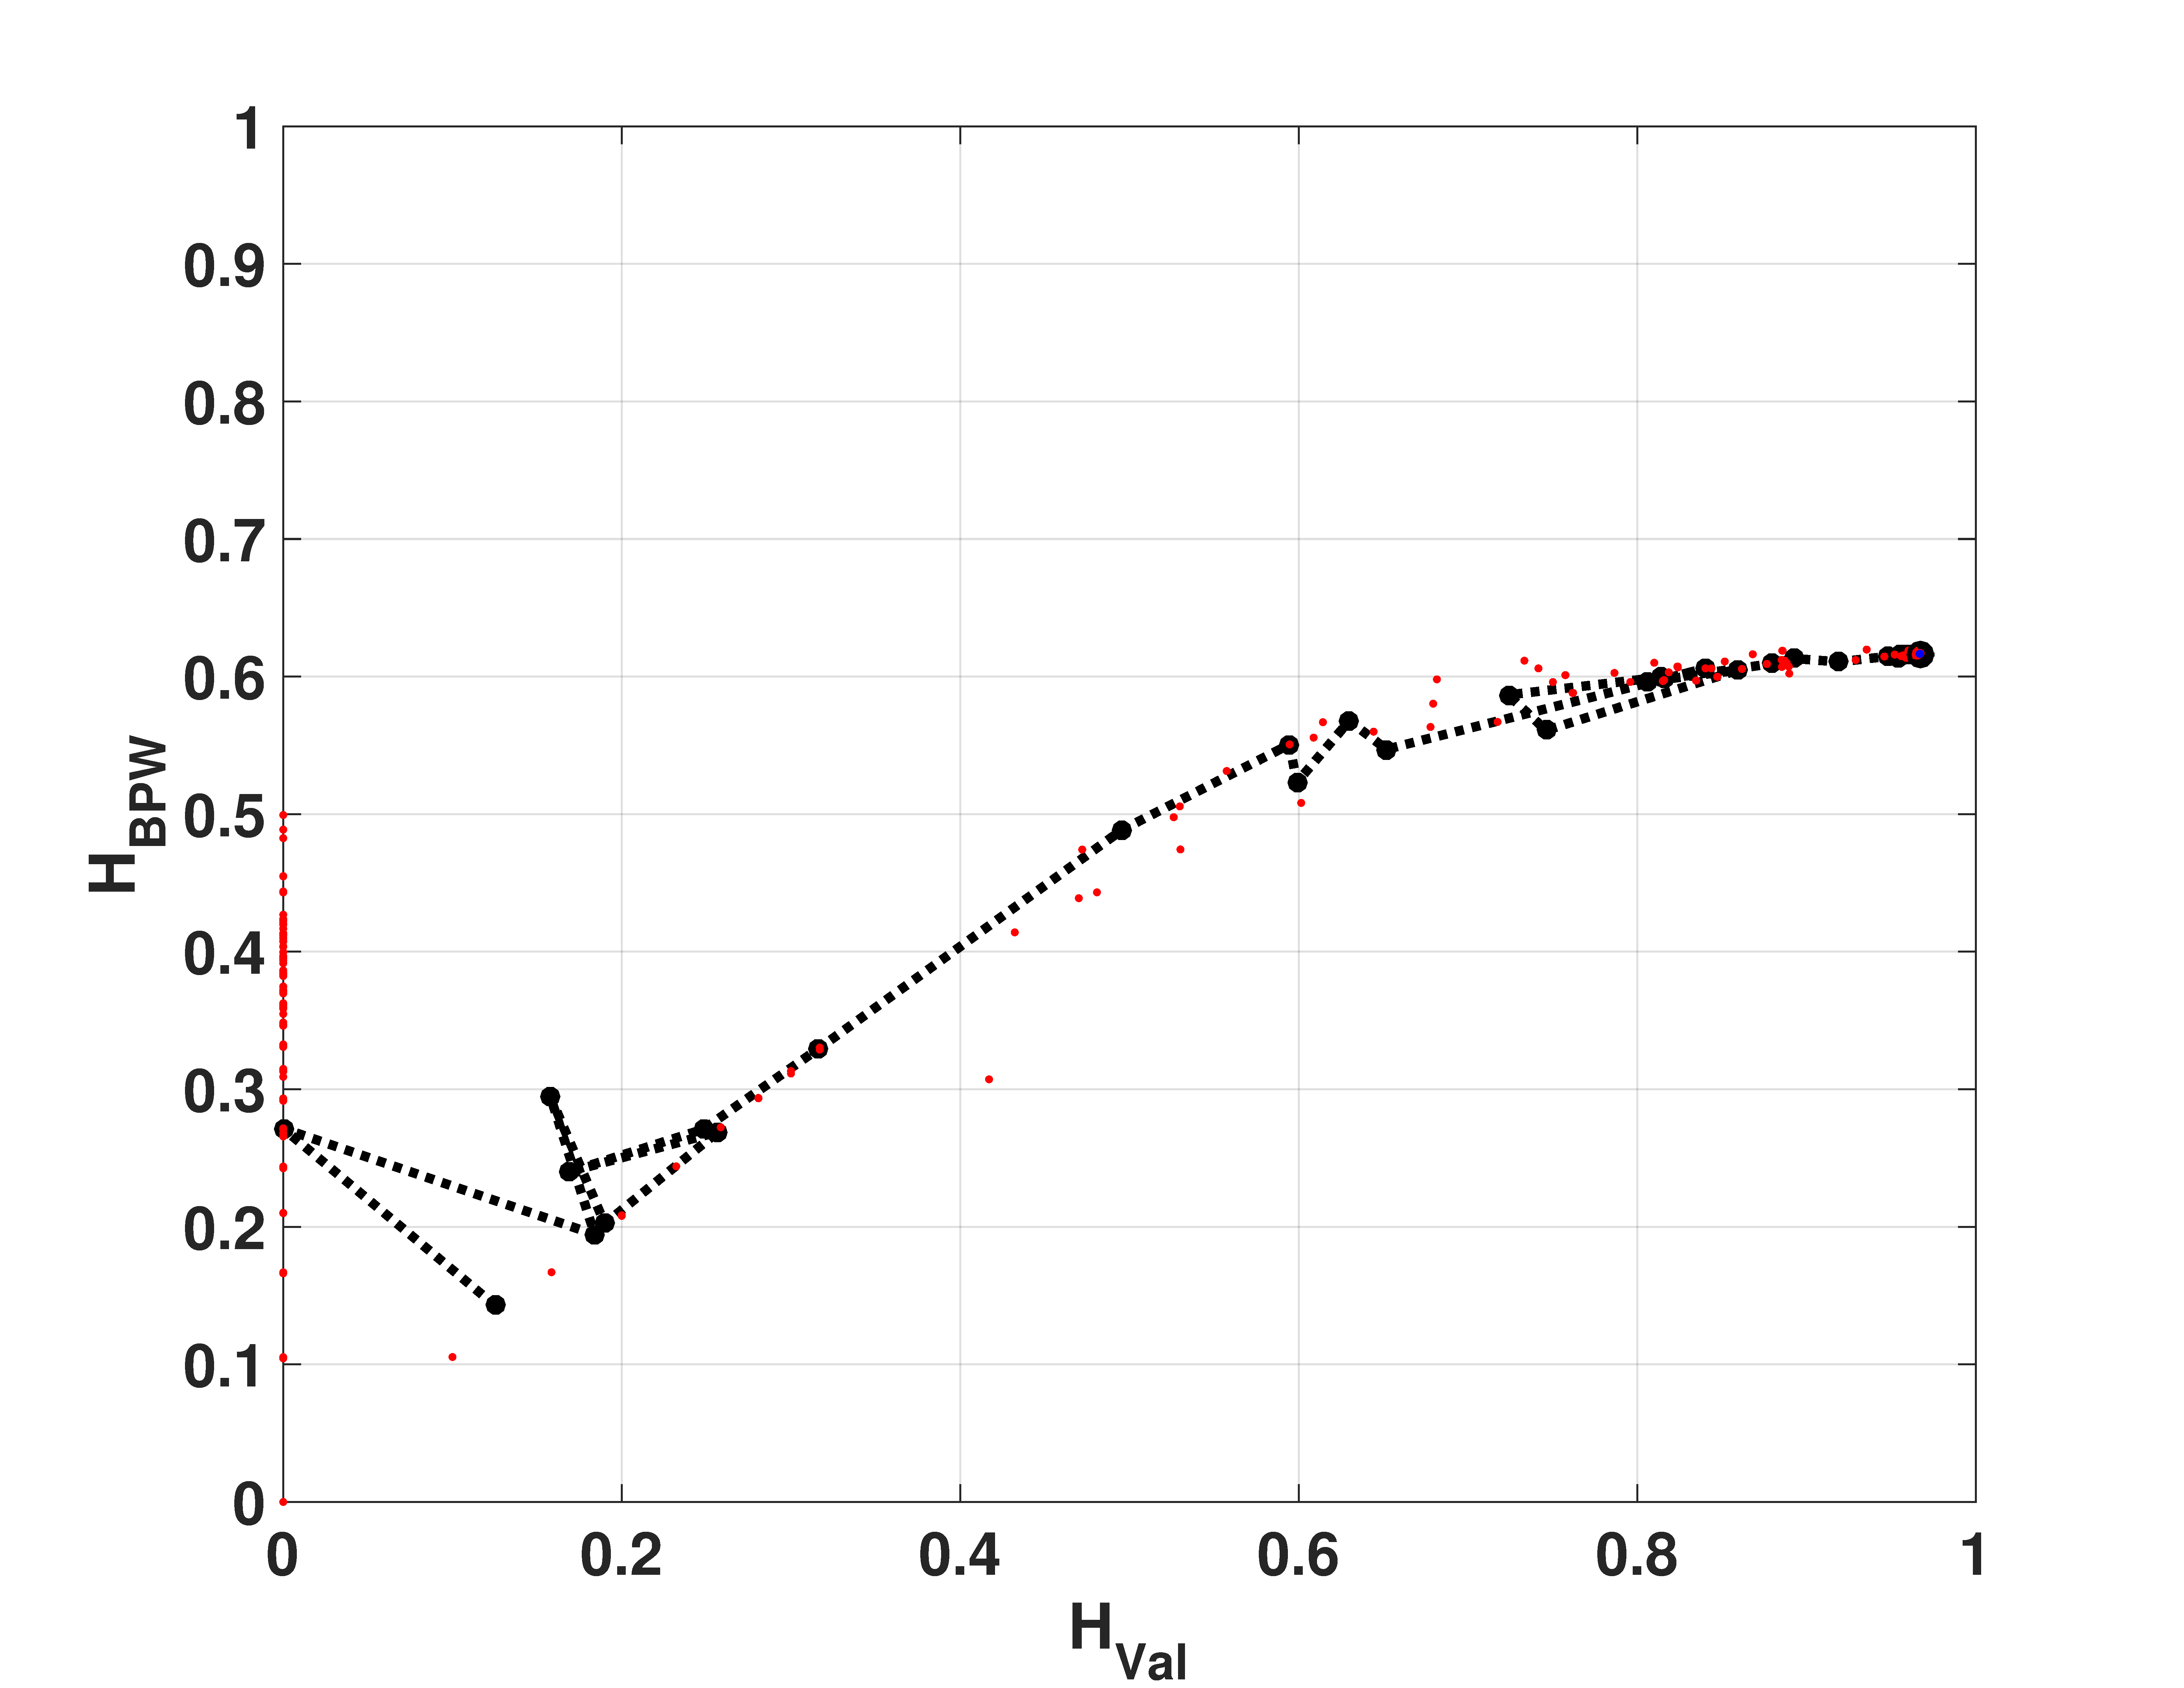
\includegraphics[width=\textwidth]{HbpwHval_Log}
		\caption{$H_{hist} \times H_{BPW}$}
		\label{fig:HbpwHbp_Log}
	\end{subfigure}
	\caption{Evolution of statistical properties in double entropy plane for LOG map}
	\label{fig:LOG_HH}
\end{figure}

In Fig. \ref{fig:LOG_HC} (a) and \ref{fig:LOG_HC} (b) we show the entropy-complexity planes.
Dotted grey lines are the upper and lower margins, it is expected that a chaotic system remains near the upper margin.
These results characterize a chaotic behaviour, in $H_{BP} \times C_{BP}$ plane we can see a low entropy and high complexity.

\begin{figure}[htpb]
	\centering
	\begin{subfigure}[b]{0.49\textwidth}
		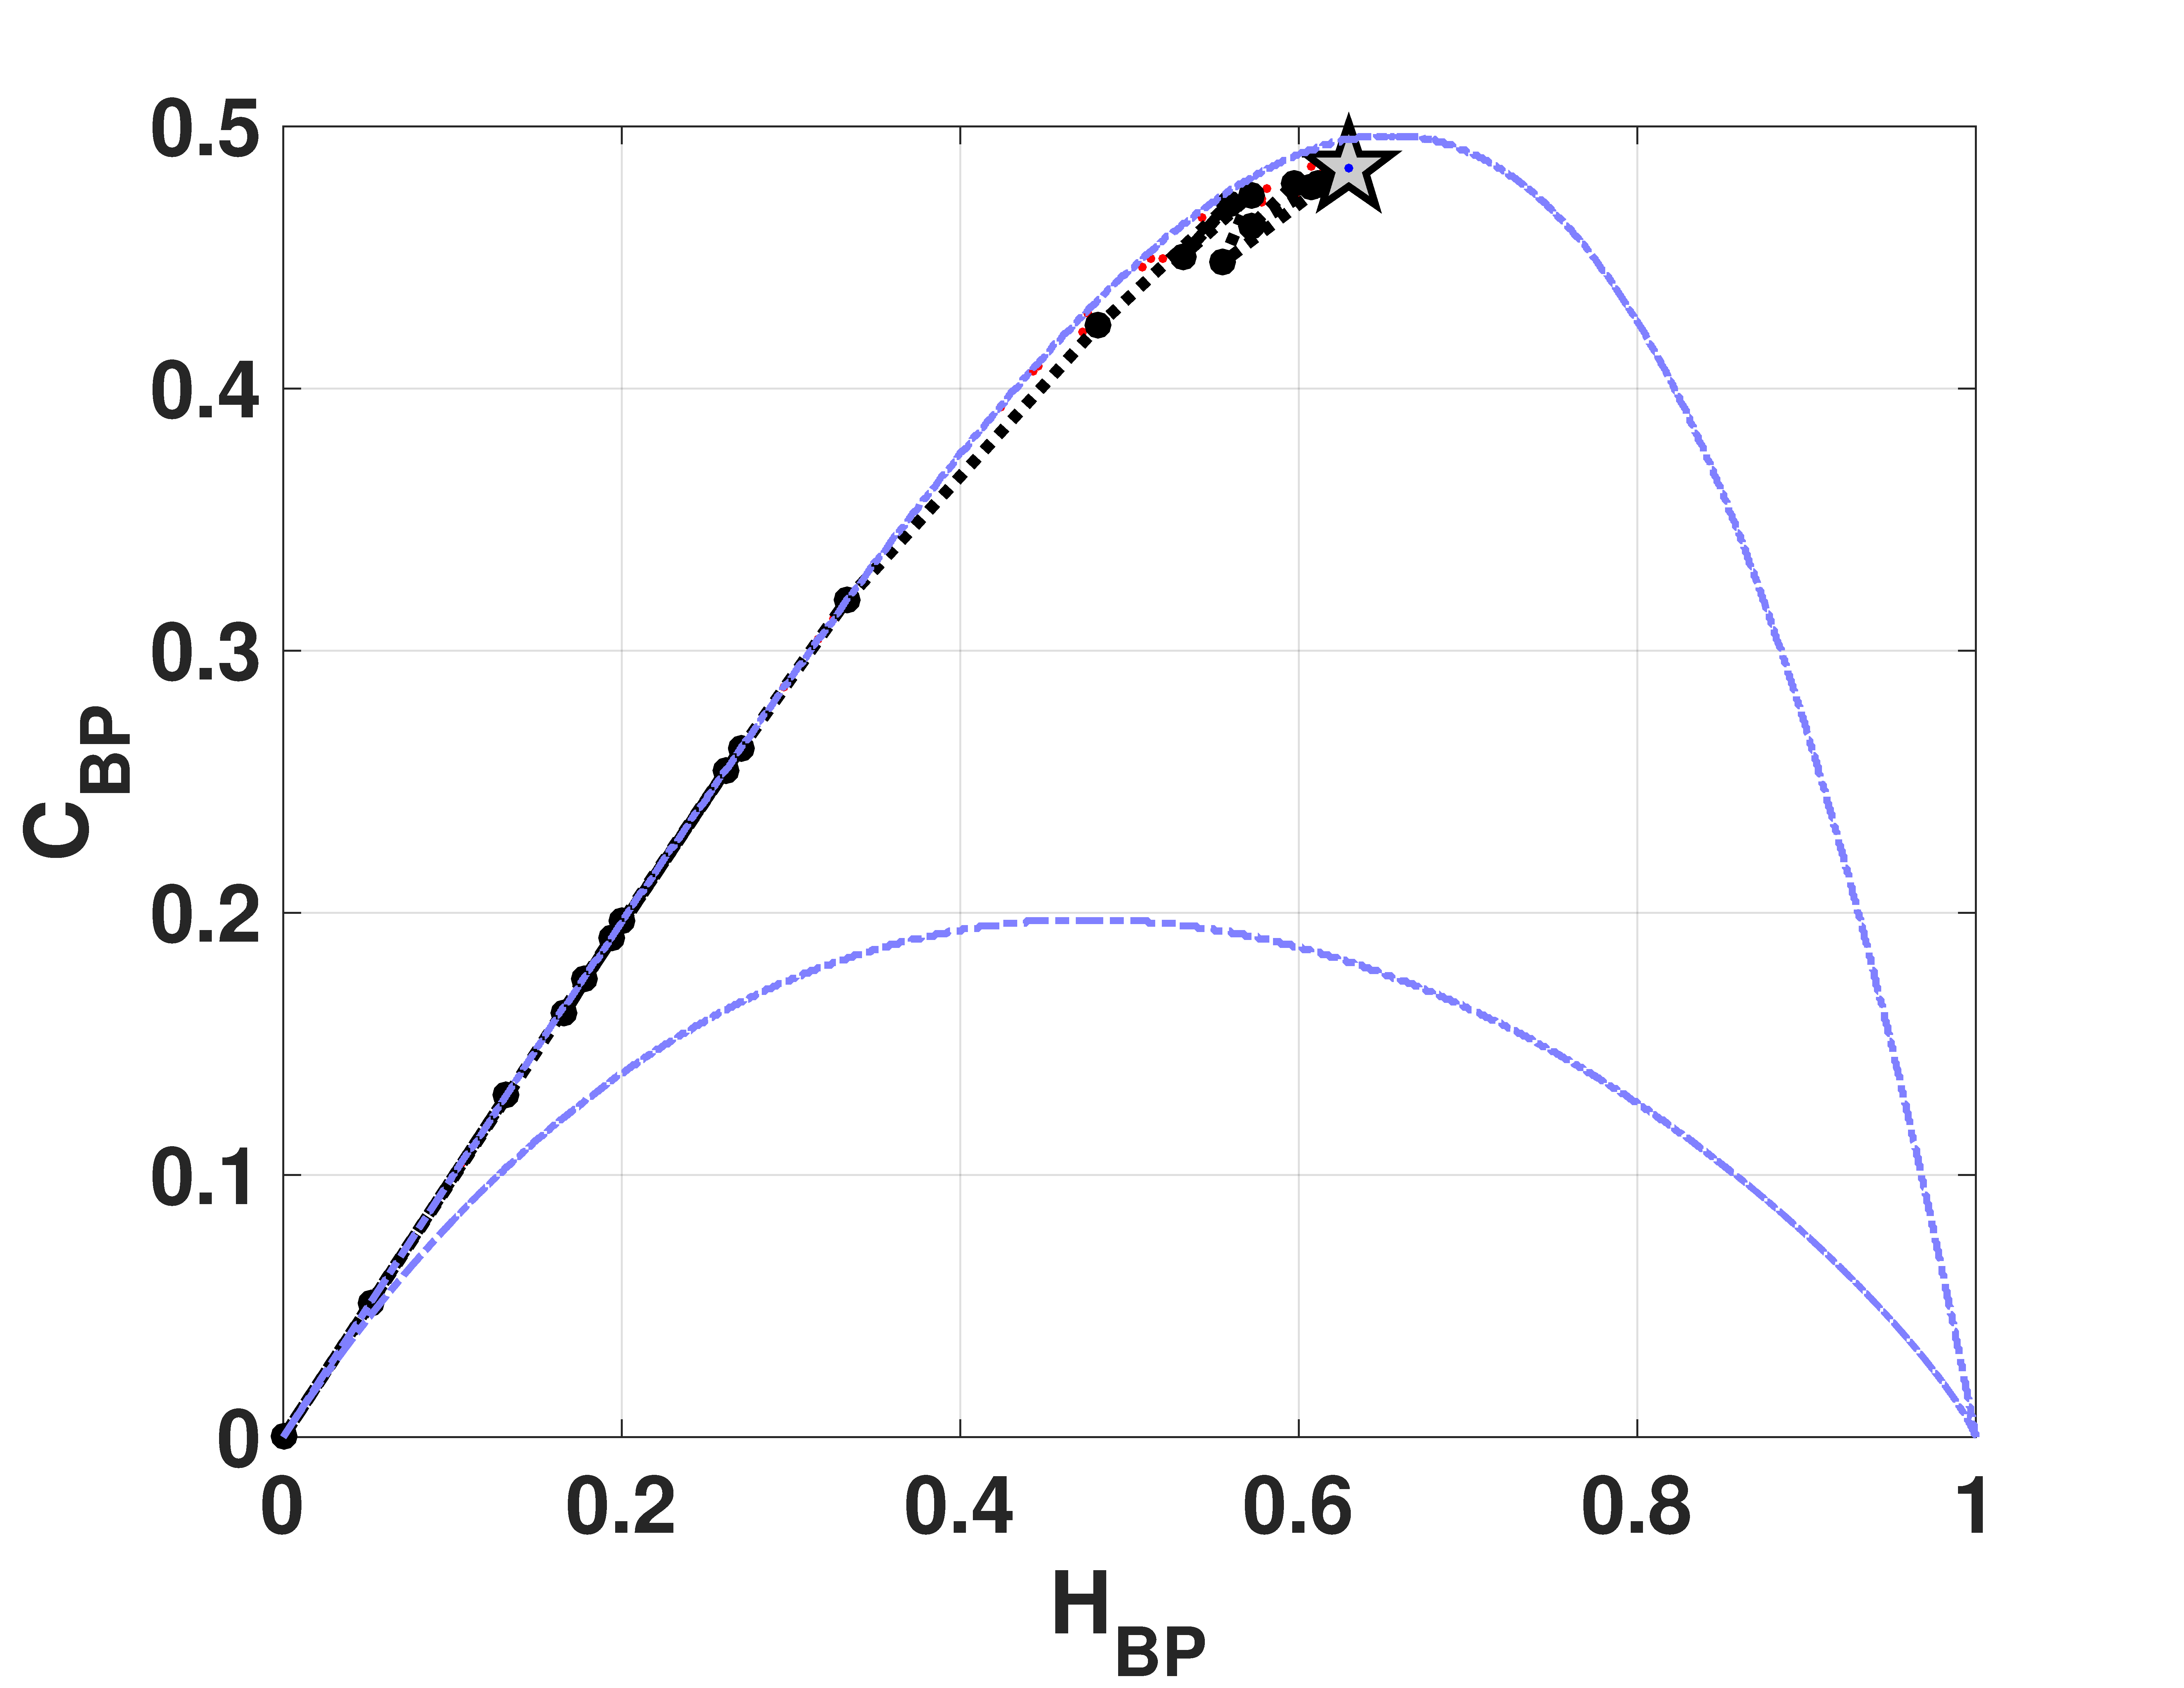
\includegraphics[width=\textwidth]{CbpHbp_Log}
		\caption{$H_{BP} \times C_{BP}$}
		\label{fig:CbpHbp_Log}
	\end{subfigure}
	\begin{subfigure}[b]{0.49\textwidth}
		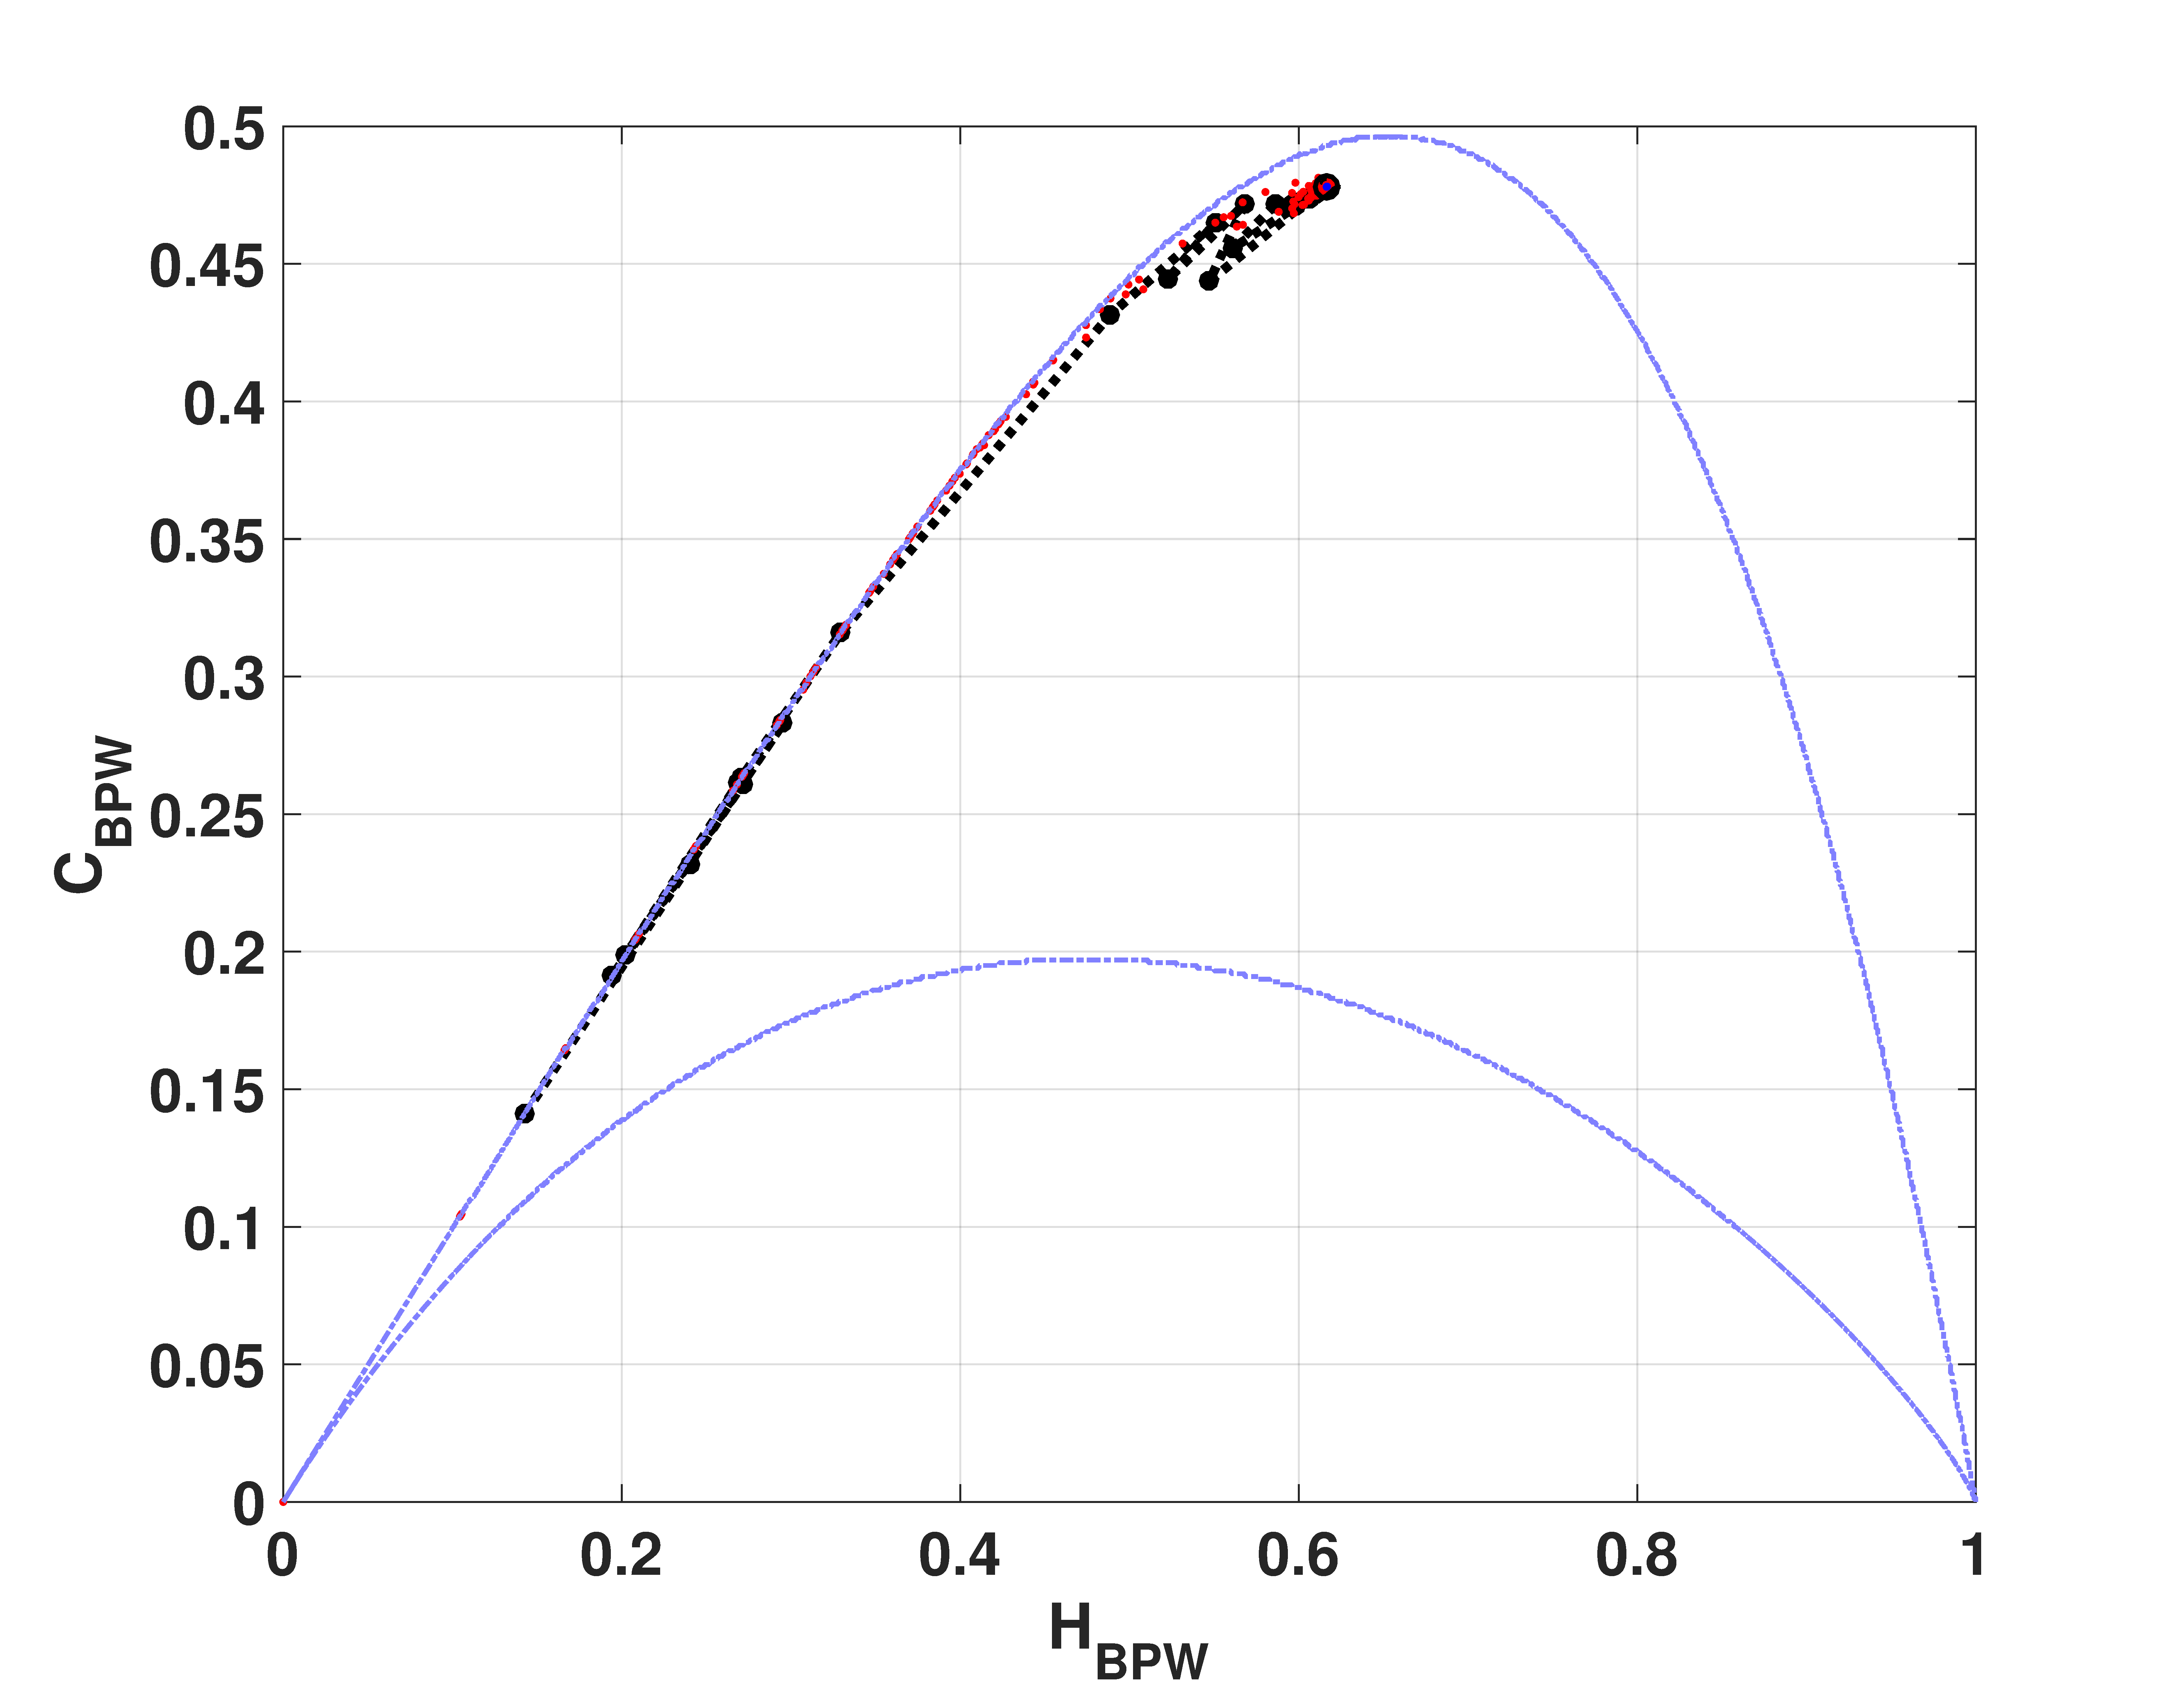
\includegraphics[width=\textwidth]{CbpwHbpw_Log}
		\caption{$H_{BPW} \times C_{BPW}$}
		\label{fig:CbpwHbpw_Log}
	\end{subfigure}
	\caption{Evolution of statistical properties in causal entropy-complexity plane for LOG map}
	\label{fig:LOG_HC}
\end{figure}
